\documentclass{thesisclass}
% Based on thesisclass.cls of Timo Rohrberg, 2009
% ----------------------------------------------------------------
% Thesis - Main document
% ----------------------------------------------------------------

\usepackage{amsmath}
\usepackage{amssymb}
\usepackage{graphicx}
\usepackage{color}
\usepackage{transparent}
\usepackage{dsfont}
\usepackage{pgfplots}

\usepackage{algorithm}
\usepackage{algpseudocode}
%\usepackage[]{algorithm2e}
%\usepackage{listings}

\usepackage{blindtext}
\usepackage{multirow}

\renewcommand{\vec}{\overline}
\renewcommand{\to}{\rightarrow}
\newcommand{\lra}{\leftrightarrow}

\newcommand{\fat}{\boldsymbol}
\newcommand{\dotp}[2]{\left\langle #1, #2 \right\rangle}
\newcommand{\dist}[2]{\left\| #1 - #2 \right\|}
\newcommand{\abs}[1]{\left| #1 \right|}

%% -------------------------------
%% |  Information for PDF file   |
%% -------------------------------
\hypersetup{
 pdfauthor={Not set},
 pdftitle={Not set},
 pdfsubject={Not set},
 pdfkeywords={Not set}
}


%% ---------------------------------
%% | Information about the thesis  |
%% ---------------------------------

\newcommand{\myname}{Alisa Jung}
\newcommand{\mytitle}{\iflanguage{english}{Irradiance Importance Sampling}{Irradiance Importance Sampling}}

\newcommand{\reviewerone}{Prof. Dr. Carsten Dachsbacher}
\newcommand{\reviewertwo}{Prof. Dr. Hartmut Prautzsch}
\newcommand{\advisor}{Dipl-Inf. Florian Simon}

\newcommand{\timestart}{02.10.2014}
\newcommand{\timeend}{02.02.2015}
\newcommand{\submissiontime}{xx.xx.xxxx}


%% ---------------------------------
%% | ToDo Marker - only for draft! |
%% ---------------------------------
% Remove this section for final version!
\setlength{\marginparwidth}{20mm}

\newcommand{\margtodo}
{\marginpar{\textbf{\textcolor{red}{ToDo}}}{}}

\newcommand{\todo}[1]
{{\textbf{\textcolor{red}{(\margtodo{}#1)}}}{}}


%% --------------------------------
%% | Old Marker - only for draft! |
%% --------------------------------
% Remove this section for final version!
\newenvironment{deprecated}
{\begin{color}{gray}}
{\end{color}}


%% --------------------------------
%% | Settings for word separation |
%% --------------------------------
% Help for separation:
% In german package the following hints are additionally available:
% "- = Additional separation
% "| = Suppress ligation and possible separation (e.g. Schaf"|fell)
% "~ = Hyphenation without separation (e.g. bergauf und "~ab)
% "= = Hyphenation with separation before and after
% "" = Separation without a hyphenation (e.g. und/""oder)

% Describe separation hints here:
\hyphenation{
% Pro-to-koll-in-stan-zen
% Ma-na-ge-ment  Netz-werk-ele-men-ten
% Netz-werk Netz-werk-re-ser-vie-rung
% Netz-werk-adap-ter Fein-ju-stier-ung
% Da-ten-strom-spe-zi-fi-ka-tion Pa-ket-rumpf
% Kon-troll-in-stanz
}


%% ------------------------
%% |    Including files   |
%% ------------------------
% Only files listed here will be included!
% Userful command for partially translating the document (for bug-fixing e.g.)
%%\includeonly{%
%%chapter1,
%%}


%%%%%%%%%%%%%%%%%%%%%%%%%%%%%%%%%
%% Here, main documents begins %%
%%%%%%%%%%%%%%%%%%%%%%%%%%%%%%%%%
\begin{document}

% Remove the following line for German text
%\selectlanguage{ngerman}
\selectlanguage{english}

\frontmatter
\pagenumbering{roman}
%% titlepage.tex
%%

% coordinates for the bg shape on the titlepage
\newcommand{\diameter}{20}
\newcommand{\xone}{-15}
\newcommand{\xtwo}{160}
\newcommand{\yone}{15}
\newcommand{\ytwo}{-253}

\begin{titlepage}
% bg shape
\begin{tikzpicture}[overlay]
\draw[color=gray]  
 		 (\xone mm, \yone mm)
  -- (\xtwo mm, \yone mm)
 arc (90:0:\diameter pt) 
  -- (\xtwo mm + \diameter pt , \ytwo mm) 
	-- (\xone mm + \diameter pt , \ytwo mm)
 arc (270:180:\diameter pt)
	-- (\xone mm, \yone mm);
\end{tikzpicture}
	\begin{textblock}{10}[0,0](4,2.5)
		
\includegraphics[width=.3\textwidth]{logos/KITLogo_RGB.pdf}
	\end{textblock}
	\changefont{phv}{m}{n}	% helvetica	
	\vspace*{3.5cm}
	\begin{center}
		\Huge{\mytitle}
		\vspace*{2cm}\\
		\Large{
			\iflanguage{english}{Bachelor Thesis of}			
												  {Bachelorarbeit\\von}
		}\\
		\vspace*{1cm}
		\huge{\myname}\\
		\vspace*{1cm}
		\Large{
			\iflanguage{english}{At the Department of Informatics}			
													{An der Fakult\"at f\"ur Informatik}
			\\
			\iflanguage{english}{Institute for Visualization and Data Analysis (IVD)}			
                {Institut f\"ur Visualisierung and Datenanalyse (IVD)}
		}
	\end{center}
	\vspace*{1cm}
\Large{
\begin{center}
\begin{tabular}[ht]{l c l}
  % Gutachter sind die Professoren, die die Arbeit bewerten. 
  \iflanguage{english}{Reviewer}{Erstgutachter}: & \hfill  & \reviewerone\\
  \iflanguage{english}{Second reviewer}{Zweitgutachter}: & \hfill  & \reviewertwo\\
  \iflanguage{english}{Advisor}{Betreuender Mitarbeiter}: & \hfill  & \advisor\\
  %\iflanguage{english}{Second advisor}{Zweiter betreuender Mitarbeiter}: & \hfill  & \advisortwo\\
  % Der zweite betreuende Mitarbeiter kann weggelassen werden. 
\end{tabular}
\end{center}
}


\vspace{2cm}
\begin{center}
\large{\iflanguage{english}{Duration}{Bearbeitungszeit}: \timestart \hspace*{0.25cm} -- \hspace*{0.25cm} \timeend}
\end{center}


\begin{textblock}{10}[0,0](4,16.8)
\tiny{ 
	\iflanguage{english}
		{KIT -- University of the State of Baden-Wuerttemberg and National Research Center of the Helmholtz Association}
		{KIT -- Universit\"at des Landes Baden-W\"urttemberg und nationales Forschungszentrum in der Helmholtz-Gemeinschaft}
}
\end{textblock}

\begin{textblock}{10}[0,0](14,16.75)
\large{
	\textbf{www.kit.edu} 
}
\end{textblock}

\end{titlepage}

\blankpage

\begin{center}
\begin{minipage}{0.7\textwidth}

\selectlanguage{english}

\chapter*{Abstract}

For many years path tracing has been a popular choice when it came to rendering photorealistic images. By combining different sampling techniques, the algorithm can be adapted to the complexity and challenges of individual scenes. That way effects like indirect lighting and caustics can be rendered realistically.

This work will introduce a new approach to include irradiance importance sampling to a regular path tracing algorithm. Before an image is rendered, the incident radiance (direct and indirect) across a scene is approximated and cached. The information from these caches can be used to generate paths with a potentially high contribution to the rendering equation. \newline
Caching and importance sampling the incident radiance enables us to compensate for some of the drawbacks of sampling paths solely according to local surface properties. This approach may also be combined with known sampling techniques, such as next event estimation or generating samples from a BSDF (bidirectional scattering distribution function), using multiple importance sampling.


\end{minipage}
\end{center}

\blankpage

\begin{center}
\begin{minipage}{0.7\textwidth}

\selectlanguage{ngerman}

\chapter*{Zusammenfassung}
\begin{otherlanguage}{ngerman}
Seit einiger Zeit zählt Path Tracing zu den beliebtesten Verfahren bei der Erzeugung fotorealistischer Bilder. Der Algorithmus kann durch Einsatz verschiedener Sampling-Techniken variiert und an die Komplexität der darzustellenden Szene angepasst werden. So sind etwa indirekte Beleuchtung und Kaustiken realistisch darstellbar.

Diese Arbeit stellt den Einsatz von Caches zur Approximation der einfallenden Beleuchtung aus verschiedenen Richtungen vor. Vor der Berechnung eines Bildes wird die einfallende Beleuchtung (direkt und indirekt) überall in der Szene approximiert und in Caches gespeichert. Diese können beim Path Tracing genutzt werden, um Pfade mit potenziell hohem Beitrag zur Rendergleichung zu erzeugen.\newline
Dadurch lassen sich manche Schwächen ausgleichen, die auftreten, wenn diese Pfade nur nach Oberflächeneigenschaften erzeugt werden. Das Verfahren lässt sich mit bekannten Sampling-Techniken wie Next Event Estimation oder klassischem Sampling nach der BSDF (bidirectional scattering distribution function) durch den Einsatz von Multiple Importance Sampling verbinden.

\end{otherlanguage}

\end{minipage}
\end{center}


%% -------------------
%% |   Directories   |
%% -------------------
\tableofcontents
\blankpage


%% -----------------
%% |   Main part   |
%% -----------------
\mainmatter
\pagenumbering{arabic}

\chapter{Introduction}

The concept of path tracing was initially introduced by Kajiya in 1986 (\cite{kajiya}), along with the rendering equation. Basically, the idea was to create paths starting from the camera and to extend these path at each surface intersection according to some sampling strategy (e.g. according to the local BSDF).\\
Over the years, several improvements to this approach were developed. Examples include next event estimation (creating direct connections from a surface point to a light source) or bidirectional path tracing (\cite{lafortune93}, \cite{lafortune96}), where paths are created not only from camera to light source, but also from light to camera. 

We will introduce a new sampling strategy for extending paths that can be combined with known sampling techniques, and evaluate if and when this strategy can improve the quality of the resulting images. Our strategy is based on caching the incident radiance, i.e. we will place caches across the scene and each of these caches will store the incident radiance for different directions, thus allowing us to sample directions from irradiance.

Chapter \ref{chapterBasics} will outline some concepts of probability theory and numerical integration, and introduce the problem of physically based light transport. In chapter \ref{chaper:PathTracing} we will introduce path tracing, a common algorithm to render photorealistic images. Chapter \ref{chapter:irradiance_caching} covers our new approach: Creating caches  that can later be used for irradiance importance sampling. In chapter \ref{chapter:rendering} we show how we combined these caches with our basic path tracing algorithm and evaluate the results. Finally, chapter \ref{chapter:relatedWork} references some related concepts.



\chapter{Basics}
\label{chapterBasics}

This chapter covers all basic concepts and definitions used in the main part of this thesis. First we will cover some probability theory and Monte Carlo integration. Furthermore we present multiple importance sampling, a common variance reduction technique to improve Monte Carlo integration. After that we will introduce physically based rendering and the rendering equation.

\section{Mathematical Basics}
\subsection{Some Probability Theory}

For all probability related concepts we use the same definitions and terminology as in \cite{veachdiss}. This section will only give a short overview on those equations that we will really need later on. For simplicity we will skip most of the derivations and equations that are not important to understand the main part of this thesis. See \cite[chapter 2.3]{veachdiss} for additional background information on probability theory.\\

\textbf{The Probability Density Function}

We will start with probability density functions (\textbf{pdf}). In general, a pdf is a continuous function $\Omega \rightarrow \mathbb{R}^+_0$ with the additional condition

\begin{equation}
\label{int_eins}
\int_\Omega p(x) dx = 1.
\end{equation}

For one-dimensional $\Omega \subseteq \mathbb{R}$, we can use $p$ to compute the probability $\mathcal{P}$ of a random variable $X$ with that density lying in an Interval $\lbrack a,b\rbrack \subseteq \Omega$ as follows:

\begin{equation*}
\mathcal{P}\{a \leq X \leq b\} = \int _a^b p(x) dx.
\end{equation*}

We can also extend this principle to $n$-dimensional $\Omega \subseteq \mathbb{R}^n$ and random variables \\$X=(X^1, \dots, X^n) \in \Omega$. At first we need the \emph{joint cumulative distribution function} $P$:

\begin{equation*}
P(X) = P(x^1,\dots,x^n) := \mathcal{P}\{X^i \leq x^i \text{ }\forall i = 1,\dots,n\}.
\end{equation*}

The \emph{joint density function} $p$ for multidimensional $\Omega$ can be obtained from

\begin{equation}
\label{p1}
p(x^1,\dots,x^n) = \frac{\partial ^n P}{\partial x^1 \cdots \partial x^n}(x^1,\dots,x^n).
\end{equation}

Note that this definition also works for $n=1$ and agrees with the conditions from above (equation \ref{int_eins}).

The joint density function $p$ can be used to compute the probability of $X$ being part of some Lebesgue measurable subset $D\subseteq \Omega$:

\begin{equation*}
\mathcal{P}\{X\in D\} = \int_D p(X)d(X) = \int_D p(x^1, \dots, x^n) dx^1 \cdots dx^n.
\end{equation*}\\

\textbf{Measures}

Throughout this thesis, we are going to use different criteria (e.g. surface area, solid angle or projected solid angle) to measure the same domain. This also affects the form of the applied pdfs. In the previous section we always integrated directly using $dx$ or $dx^i$. We will now introduce a more general approach that allows us to transform between different measures.

First of all, we define

\begin{equation*}
P(D) := \mathcal{P}\{X\in D\}.
\end{equation*}

$P$ is a measure function called \emph{probability measure} for a random variable $X \in \Omega$. Just as in equation \ref{int_eins}, we demand $P(\Omega) = 1$. Similar to equation \ref{p1}, we obtain a corresponding pdf $p$ depending on a measure $\mu$ as follows:

\begin{equation}
\label{def_p}
p(x) = \frac{dP}{d\mu}(x).
\end{equation}

There are different ways to pick $D$ and $\mu$ and therefore different possible pdfs. All of them satisfy

\begin{equation*}
P(X) = \int_Dp(x)d\mu(x)
\end{equation*}

with their very own measure $\mu$ that was used to define them in \ref{def_p}.\\

\textbf{Expectation and variance}

The \emph{expectation} or \emph{expected value} $E$ of a random variable $X$ with density $p$ and measure $\mu$ represents the expected average value of a huge number of random variables with density $p$. It is defined as

\begin{equation*}
E(X) = \int_\Omega x \cdot p(x) d\mu(x).
\end{equation*}

This equation also works if we consider some function $f$ of $X$ instead of $X$ itself:

\begin{equation*}
E(f(X)) = \int_\Omega f(x) \cdot p(x) d\mu(x).
\end{equation*}

The \emph{variance} indicates how much the random variables vary from the expected value. A variance of $0$ means that all random variables equal the expectation. The variance is always greater than or equal to zero and given by

\begin{equation*}
Var(X) = E\lbrack(X-E(X))^2\rbrack.
\end{equation*}

Another measure for the variation of random variables is the \emph{standard deviation}:

\begin{equation*}
\sigma(X) = \sqrt{Var(X)}.
\end{equation*}

\subsection {Monte Carlo Integration}
Monte Carlo integration is a non-deterministic unbiased numerical method for estimating integrals and is especially useful whenever those integrals are high dimensional. As explained later on, solving the light transport problem requires computing such an integral over a theoretically infinite number of dimensions. We will now present the Monte Carlo estimator, show some of its advantages and introduce importance sampling to improve it.

Say we want to integrate a function $f:\Omega \rightarrow \mathbb{R}$ over $\Omega$, where $\Omega$ has an arbitrary dimensionality and $\mu$ is some measure function on $\Omega$:

\begin{equation}
\label{int f}
I = \int_\Omega f(x) d\mu(x).
\end{equation}

Let $p(x)$ be a probability density function on $\Omega$ with 

\begin{equation*}
\forall x \in \Omega: f(x) \neq 0 \Rightarrow p(x) > 0
\end{equation*}

and let $X$ be a random variable with density $p$. Then we can also express $I$ as follows:

\begin{equation*}
I = \int_\Omega f(x) d\mu(x) = \int_\Omega \frac{f(X)}{p(X)} \cdot p(X) d\mu(X) = E\left(\frac{f(X)}{p(X)}\right).
\end{equation*}

Thus we can interpret $I$ as the expectation of $f(X)/p(X)$. This expected value can be approximated using the Monte Carlo estimator $F_N$:

\begin{equation}
\label{f_n}
I = E\left(\frac{f(X)}{p(X)}\right) \approx \frac{1}{N}\sum_{i = 1}^N \frac{f(X_i)}{p(X_i)} =: F_N.
\end{equation}

We use the index $N$ to indicate that the estimator uses $N$ samples.\\

\textbf{Error and Bias}

Given an estimator $F_N$ and the quantity $I$ we want to estimate, $F_N - I$ is called the \emph{error} of the estimator. The \emph{bias} $\beta$ of an estimator is the expected value of its error:

\begin{equation*}
\beta\lbrack F_N\rbrack = E(F_N - I).
\end{equation*}

If $\beta\lbrack F_N\rbrack = 0$ independent of the number of samples $N$, the estimator is called \emph{unbiased}. This is a desirable property for any estimator, because it guarantees that it will yield the correct value on average.\\

\textbf{Advantages of Monte Carlo integration}

The Monte Carlo estimator is unbiased, since

\begin{equation*}
\beta\lbrack F_N\rbrack = E\left( \frac{1}{N}\sum_{i = 1}^N \frac{f(X_i)}{p(X_i)} - I\right) = E\left( \frac{1}{N}\sum_{i = 1}^N \frac{f(X_i)}{p(X_i)}\right) - E(I) =  E\left(\frac{f(X)}{p(X)}\right) - I = I-I = 0.
\end{equation*}

When dealing with one or two dimensions, other techniques such as quadrature rules perform way better than $F_N$. However, Monte Carlo integration is practically the only integration method hat can handle infinite-dimensional integrals at all. \\
It also has some desirable properties when dealing with high-dimensional integrals. First of all, its quality does not depend on the dimensionality. With deterministic approaches, the number of samples needed for the same standard deviation explodes exponentially with each additional dimension. In contrast, the standard deviation of $F_N$ is always proportional to $1/\sqrt{N}$, regardless of the dimensionality. More precisely,

\begin{equation}
\label{deviation}
\sigma(F_N) = \frac{1}{\sqrt{N}}\sigma \left(\frac{f(X)}{p(X)}\right),
\end{equation}
as elaborated in \cite{veachdiss}. The quality of the estimator solely depends on the number of samples and on the quality of $p$ (i.e. how proportional $p$ and $f$ are). The estimator also converges at a rate of $\mathcal{O}(1/\sqrt{N})$.

Another advantage of Monte Carlo integration is its ability to handle singularities, i.e. functions with discontinuities. In computer graphics, this is the case with ideal specular surfaces (e.g. mirrors), where light arriving from one direction is only scattered along exactly one outgoing direction; in other words, only light from one single direction contributes to the color we see on that surface.

See \cite[chapter 2]{veachdiss} for additional information on Monte Carlo integration.\\


\textbf{Importance Sampling}

The difficulty of Monte Carlo integration lies in finding a good pdf. It can be shown that the optimal choice is 
\begin{equation*}
p^*(x) = \frac{f(x)}{I}
\end{equation*}

with a derivation of $0$ (see equation \ref{deviation} and \cite[chapter 2.5.2]{veachdiss}) - one sample generated by $p^*$ would suffice to compute the exact value of $I$. Unfortunately, since $I$ is the value we want to approximate, we can't know the exact value of $I$ in advance (if we did, numerically approximating $I$ would be pointless).\\
However, there are ways to quickly construct a pdf that is at least roughly proportional to $f$. Generating Samples from a probability density function that is supposedly proportional to $f$ is called \emph{Importance Sampling}. Section \ref{importance_sampling_options} shows some Importance Sampling strategies specifically designed for approximating the rendering equation.

Importance Sampling is one of several so-called \emph{variance reduction methods}. In addition to Importance Sampling we only used Russian Roulette, which is explained in section \ref{chapterRussianRoulette}. See \cite[chapters 2.5 - 2.8]{veachdiss} for an introduction to other variance reduction methods.


\subsection{Multiple Importance Sampling}
\label{multiple importance sampling}
It can be hard to construct one general pdf that performs well in any case. Most times, it is easier to construct different pdfs that perform well under different circumstances, and weight them together. This can greatly improve Importance Sampling and is called \emph{Multiple Importance Sampling (MIS)}.

As we will see in section \ref{importance_sampling_options}, there are different strategies to create pdfs for physically based rendering, but all of them show major weaknesses under different conditions. We will now show how any sampling strategies can be combined in a way that, given a pdf $p$ ($p'$) that performs well (badly) in case A and badly (well) in case $B$, whenever we have case A $p$ is chosen more often or weighted more heavily than $p'$. Thus we can reduce variance and make Monte Carlo integration more robust.

There are two main categories for MIS: The multi-sample model, where many samples are generated and weighted together for one step, and the one-sample model, where only one sample is generated per step, which means we have to pick and weight one pdf for every step.

Given a domain $\Omega$, a function $f:\Omega \rightarrow \mathbb{R}$ and a measure $\mu$, both models use a set of $n$ sampling strategies with pdfs $p_1 , \dots, p_n$ to approximate equation \ref{int f}.

In order to apply the models, $f(x)$ and $p_i(x)$ must be defined for any $x\in \Omega, i\in 1, \dots, n$, and we have to be able to generate samples from $p_1, \dots, p_n$.\\


\textbf{The Multi-Sample Model}

The multi-sample model can be applied whenever we are able to generate one or more samples from each sampling strategy ($=$ pdf) to approximate an integral.

First, a fix number $n_i\geq 1$ of samples is generated from each sampling strategy $i$ according to its pdf $p_i$. We will denote each sample $X_{i,j}$ with $i = 1,\dots ,n$ and $j=1,\dots,n_i$ referring to the sampling strategy and its number of samples respectively.\\
All samples generated from the same strategy $i$ share one weighting function $w_i$. This allows us to assign different weights to samples from the same strategy. Finally we can compute the \emph{multi-sample estimator} $F$ to approximate \ref{int f}:

\begin{equation*}
F=\sum_{i=1}^n \frac{1}{n_i} \left( \sum_{j=1}^{n_i} w_i(X_{i,j}) \frac{f(X_{i,j})}{p_i(X_{i,j})} \right).
\end{equation*}

If we want $F$ to be unbiased (\cite[Lemma 9.1]{veachdiss}), there are two conditions for our weighting functions:

\begin{equation}
\label{condw1}
f(x) \neq 0 \Rightarrow \sum_{i=1}^n w_i(x) = 1 \text{ and}
\end{equation}

\begin{equation}
\label{condw2}
\forall i = 1, \dots, n: p_i(x) = 0 \Rightarrow w_i(x) = 0.
\end{equation}

Note that for $n=1, n_1 = N$ and $w_1(x) = 1/N$ (one pdf with $N$ uniformly weighted samples) the resulting estimator $F$ equals $F_N$ from equation \ref{f_n}.

Path tracing usually uses the multi-sample model to combine BSDF sampling and next event estimation, a short overview on that case is given in section \ref{pathtracingalgorithm}.\\



\textbf{The Balance Heuristic}

One possible way to define the weighting functions is

\begin{equation}
w_i(x) = \frac{n_ip_i(x)}{\sum_k n_kp_k(x)}.
\end{equation}

This combining strategy is called \emph{balance heuristic}. It shows a minimal variance compared to any other combination strategy -  \cite[9.2.2, page 264]{veachdiss} shows that ``no other combination strategy is much better''.\\


\textbf{The Power Heuristic}

The power heuristic is a generalization of the balance heuristic. It uses an exponent $\beta$ for all weights:

\begin{equation}
\label{power heuristic}
w_i(x) = \frac{(n_ip_i(x))^\beta}{\sum_k (n_kp_k(x))^\beta}.
\end{equation}

As Veach showed in \cite[chapter 9.3.1]{veachdiss}, the power heuristic for $\beta=2$ can lead to better results for very rough or barely rough surfaces.

Other possible weighting functions include discrete $w_i(x) \in \{0,1\}$ or uniform functions $w_i(x) = 1/n$, the cutoff heuristic, which ignores samples with small probabilities, or the maximum heuristic (the power heuristic for $\beta \rightarrow \infty$).\\

\textbf{The One-Sample Model}

There are times when we cannot or do not want to generate multiple samples from multiple pdfs, but still have several sampling strategies to choose from. In that case, we use a set of fix probabilities $c_1, \dots c_n$ with $\sum c_i = 1$ to pick one of our $n$ sampling strategies and take one sample $X_j$ from the chosen pdf $p_j$. The \emph{one-sample estimator} to approximate \ref{int f} is given as

\begin{equation}
\label{onesample}
F=\frac{w_j(X_j)f(X_j)}{c_jp_j(X_j)}.
\end{equation}

For this model the balance heuristic is such a good choice for the weighting function that we don't have to use any improvements like the power heuristic (\cite[9.2.4]{veachdiss}). Plus, as long as we consider conditions \ref{condw1} and \ref{condw2}, equation \ref{onesample} also gives an unbiased estimator.

In section \ref{mis_BSDF_irc}, we will use the one-sample model to combine two different sampling strategies for extending a path. We will also decide on $c_1$ and $c_2$ depending on the current surface probabilities instead of using the same $c_1$ and $c_2$ every time.


















\newpage
\section{Physically based light transport}

\subsection{Assumptions}
Before we introduce the equations we used to model light transport, we are going to make a few assumptions. These constraints won't produce any significant difference compared to a physically accurate model, as long as we only render ``ordinary'' scenes that don't rely heavily on one of the excluded phenomena. However, it is always important to decide if the current model can produce valid results for a certain scene, or if some of those assumptions have to be discarded.

Basically we assume a geometric optics model, where light only travels in straight lines and only interacts (gets emitted, scattered or absorbed) at surfaces. We also ignore all behaviour that arises from the wave or quantum characteristics of light.\\
Thus the proposed model can't accurately render phenomena like participating media (e.g. fog or smoke), subsurface scattering (e.g. wax) or relativistic effects, diffraction or fluorescence. It also ignores varying refraction indices, be it dispersion at a surface, caused by a different index for different wave lengths, or media with a continuously varying index. With this model, light of any wavelength behaves the same, and no energy is lost while traveling between surfaces.

There are some additional choices caused by the Mitsuba Renderer \cite{mitsuba} which we used as an implementation framework. Mitsuba supports a wide range of surfaces scattering models (see \cite[Mitsuba Documentation chapter 8.2]{mitsuba}) and allows for transmitting and ideal specular surfaces. However, in our implementation and test scenes, we ignored the more complex BSDFs for simplicity. We also ignore point light sources and terminate any path as soon as it hits a light source.

\newpage
\subsection{Notations}
From now on, we will use the following notations (depicted in figure \ref{hemi}):
\begin{itemize}
\item $\mathcal{S}^2$ will be the set of all directions.
\item $\omega \in \mathbb{R}^3$, $||\omega|| = 1$ will describe any direction on the unit sphere.
\item $x$ will refer to a surface point and $N(x)$ to the surface's normal at $x$.
\item $\sigma$ is the surface area measure on $\mathcal{S}^2$.\\
$\sigma(\omega)$ represents the solid angle covered by $\omega$.
\item $\sigma^\bot_x(\omega) := |\omega \cdot N(x)| \cdot \sigma(\omega)$ is the projected solid angle at $x$.\\
Sometimes we might just use $\sigma^\bot(\omega)$ to refer to projected solid angles in general.\\
Note that the solid angle and projected solid angle are unitless.
\item $dA(x)$ will refer to an infinitesimal surface area around $x$.
\item $\mathcal{H}_+^2(x) = \{\omega\in\mathcal{S}^2 | \omega \cdot N(x) > 0\}$ is the upper hemisphere and

$\mathcal{H}_-^2(x) = \{\omega \in\mathcal{S}^2 | \omega \cdot N(x) < 0\}$ is the lower hemisphere at $x$.
\item $L_o(x,\omega)$ represents the radiance leaving $x$ into direction $\omega$.
\item $L_i(x,\omega)$ represents the incoming radiance at $x$ from direction $\omega$.
\item $ray(x,\omega)$ refers to a ray with origin $x$ and direction $\omega$.
\item $x_\mathcal{M}(x,\omega)$ is the \emph{ray casting function}. It returns the first surface point that is hit by $ray(x,\omega)$.


\end{itemize}
In free space (where $x$ is not a surface point) $L_i(x,\omega) = L_o(x,-\omega)$. At surfaces the relation between $L_i$ and $L_o$ is more complex, see section \ref{rendering equation}.

Also note that for $L_i(x,\omega_i)$ the photons are actually moving in direction $-\omega_i$, as the $\omega \in \mathbb{R}^3$ always point from $x$ towards the hemisphere while the (incident) photons move through the hemisphere towards $x$.


\begin{figure}[ht]
	\centering
\def\svgwidth{380pt}
  \input{hemispheretext.pdf_tex}
	\caption{The upper blue line represents $\mathcal{H}^2_+$, the dotted blue line represents $\mathcal{H}^2_-$.}
\label{hemi}\end{figure}

\newpage
\subsection{Radiometry}

This section will briefly cover the physical background of radiance and irradiance.\\
 Physically speaking, the \emph{irradiance} is defined as power $\Phi$ (in Watt) per unit surface area $A$ (in $m^2$) at some point $x\in\mathbb{R}^3$:

\begin{equation*}
E(x) = \frac{d\Phi(x)}{dA(x)}.
\end{equation*}

The term irradiance and $E$ are used for the total \emph{incident} radiation on \emph{one} hemisphere only. Radiance \emph{leaving} the surface is referred to as \emph{radiant exitance} and can happen on both hemispheres. 

The \emph{radiance} itself can be expressed as

\begin{equation*}
L(x,\omega) = \frac{d^2\Phi(x,\omega)}{dA(x)d\sigma^\bot_x(\omega)}.
\end{equation*}

It measures the radiance at $x$ from an infinitesimal cone around direction $\omega$. The definition of $L$ can also be extended to include different wavelengths; we will ignore that.\\
We will use $\omega_i$ and $L_i(x,\omega_i)$ to refer to radiance arriving at a point $x$ from direction $\omega_i$ (photons moving along $-\omega_i$), and $L_o(x,\omega_o)$ when we talk about the radiance leaving $x$ into direction $\omega_o$.


We can also express irradiance as an integral of incoming light as follows:

\begin{equation*}
E(x) = \int_{\mathcal{H}^2_+(x)}L(x,\omega)d\sigma^\bot(\omega)
\end{equation*}
or
\begin{equation}
\label{e and l}
dE(\omega_i) = L_i(\omega_i)d\sigma^\bot(\omega_i).
\end{equation}

Experiments have shown that irradiance and outgoing radiance are proportional, i.e. 

\begin{equation*}
dL_o(\omega_o) \propto dE(\omega_i).
\end{equation*}

We will not explain this topic any further, see \cite[chapter 9.3]{veachdiss} for a more detailed introduction on radiometric quantities.\\


\subsection{The bidirectional scattering distribution function (BSDF)}
\label{BSDF}

The \emph{bidirectional scattering distribution function} (\textbf{BSDF}) is used to describe how surfaces scatter light. It indicates how much of the energy arriving at a point $x$ from an incoming direction $\omega_i$ is scattered into any outgoing direction $\omega_o$. 

Usually, the BSDF is divided into a \emph{bidirectional reflectance distribution function} (BRDF) and a \emph{bidirectional transmittance distribution function} (BTDF), that cover the reflectance and transmittance at a surface respectively. The BRDF only uses incoming and outgoing directions on the same hemisphere, whereas the BTDF only uses directions on opposite hemispheres. Since the BSDF is simply the union of two BRDFs and two BTDF (one for each side of the surface), we will only use the BSDF later on. We will denote BRDFs with $f_r$, BTDFs with $f_t$ and BSDFs with $f_s$.\\

\textbf{Parameterization}

The BSDF $f_s$ at some surface point $x$ is defined as

\begin{equation*}
f_s(\omega_i,x,\omega_o) = \frac{dL_{o,s}(\omega_o)}{dE(\omega_i)}.
\end{equation*}

Using equation \ref{e and l} we can also write $f_s$ as
\begin{equation}
\label{scattering1}
f_s(\omega_i,x,\omega_o) = \frac{dL_{o,s}(\omega_o)}{L_i(\omega_i)d\sigma^\bot(\omega_i)}.
\end{equation}

It describes the relation of radiance arriving from direction $\omega_i$ to $L_{o,s}(x,\omega_o)$ (radiance scattered along $\omega_o$). We add the index $s$ to $L_o$ to indicate that we are only considering outgoing light that was scattered, and ignore outgoing light that was emitted at $x$.

With physically based rendering, we can always assume that the incoming radiance originated at some point $x_0$ (either it was emitted at $x_0$ along $-\omega_i$ and hit $x$ directly, or it was emitted somewhere else, scattered across the scene and finally scattered from $x_0$ to $x$).\\
Theoretically a ray with origin $x$ and direction $\omega_o$ may never intersect any geometry again, which means that light scattered along $\omega_o$ leaves the scene, but those cases are not interesting for us. So, assuming that the light scattered at $x$ along $\omega_o$ hits the scene again at some point $x_2$, we can also use the following notation for $f_s$:

\begin{equation}
\label{fspoint}
f_s(x_0 \rightarrow x \rightarrow x_2) = f_s(\omega_i,x,\omega_o).
\end{equation}

\textbf{Properties}

We can make two assumptions about physically correct BRDFs that do not necessarily apply to BTDFs and BSDFs. First of all, physically correct BRDFs are always symmetric:

\begin{equation*}
\forall x, \omega_i,\omega_o: \text{ } f_r(\omega_i, x, \omega_o) = f_r(\omega_o, x, \omega_i).
\end{equation*}

Plus, we can assume that the scattered energy never exceeds the incoming energy, this property is called \emph{energy conservation}:

\begin{equation*}
\forall \omega_i \in \mathcal{H}_i^2: \text{ } \int_{\mathcal{H}_o^2}f_r(\omega_i , x, \omega_o) d\sigma^\top(\omega_o) \leq 1 .
\end{equation*}

With some surfaces these conditions do not hold for the BSDF or BTDF. To include such surfaces to a bidirectional path tracing algorithm or path tracing combined with photon mapping, we also have to use the \emph{adjoint BSDF}, which is basically the BSDF with switched arguments ($f_s(\omega_o,x,\omega_i)$ instead of $f_s(\omega_i,x,\omega_o)$, see \cite[chapter 3.7.3 - 3.7.6]{veachdiss}).\\
The adjoint BSDF is used to sample paths that carry importance and for scattering photons, while we can use the original BSDF for paths that carry radiance. Later on, we will use the adjoint BSDF in our photon mapping step, as explained in section \ref{modified photon mapping}.\\

\textbf{Delta-BSDFs}

Ideal specular surfaces have the unique property that for every outgoing direction $\omega_o$ there is exactly one incoming direction $\omega_i$, so that all of the radiance arriving at $\omega_i$ is scattered along $\omega_o$. For a given $x$ and $\omega_o$ (or $x$ and $\omega_i$), the BSDF describing this surface is always $0$ except for one $\omega_i$ (or $\omega_o$). We call such a BSDF a \emph{delta-BSDF}. All other BSDFs contain a diffuse component, we call those \emph{smooth} BSDFs.


\newpage
\subsection{The Rendering Equation}

The goal of our algorithm is to render an image, which means we have to compute the color of each individual pixel. In order to do that we model each pixel $j$ as a hypothetical sensor with area $\mathcal{M}$. The so-called \emph{sensor sensitivity function} $W_e^j(x,\omega)$ describes how this sensor responds to light arriving at $x\in \mathcal{M}$ from direction $\omega$. The color of the pixel is given as the total sensor response, called the \emph{measurement equation}:

\begin{equation}
\label{measurement equation}
I^j = \int_{\mathcal{M}\times\mathcal{S}^2}W^j_e(x,\omega)L_i(x,\omega)dA(x)d\sigma^\bot_x(\omega).
\end{equation}

Sometimes the scenes we want to render are "open" - for some directions $\omega'$ and starting points $x'$, $ray(x',\omega)$ may never intersect any geometry. This means that no light $L_i$ can arrive at $x'$ along $\omega'$ and the integrand will be $0$ for $\omega'$. For all other directions there has to be one point $x_\mathcal{M}(x,\omega)$ in the scene that was hit by a ray from $x$ along $\omega$.

Since our model only allows light to change at surfaces, we can express the incident radiance as

\begin{equation*}
L_i(x,\omega) = L_o(x_\mathcal{M}(x,\omega),-\omega).
\end{equation*}

The outgoing light can be divided into scattered and emitted light:

\begin{equation*}
L_o(x,\omega) = L_e(x,\omega) + L_{o,s}(x,\omega).
\end{equation*}

The emitted light $L_e(x,\omega)$ is given by the scene description. We can obtain the scattered light when we convert equation \ref{scattering1} to the \emph{(surface) scattering equation}:

\begin{equation}
\label{scattering equation}
L_{o,s}(x,\omega) = \int_{\mathcal{S}^2}  L_i(x,\omega_i) \cdot f_s(\omega_i,x,\omega_o) d\sigma^\bot(\omega_i).
\end{equation}

Combining these equations leads to the \emph{rendering equation}

\begin{equation}
\label{rendering equation}
L_o(x,\omega) = L_e(x,\omega) + \int_{\mathcal{S}^2}L_i(x,\omega) \cdot f_s(\omega_i,x,\omega_o)d\sigma^\bot(\omega_i).
\end{equation}

Veach \cite[chapter 3.7.2]{veachdiss} uses the term \emph{light transport equation} for a slightly different form of the same equation:

\begin{equation*}
L_o(x,\omega_o) = L_e(x,\omega_o) + \int_{\mathcal{S}^2} L_o(x_\mathcal{M}(x,\omega_i),-\omega_i) \cdot f_s(\omega_i,x,\omega_o)d\sigma^\bot_x(\omega_i).
\end{equation*}

In theory the rendering equation (or the light transport equation) could now be solved recursively. In praxis they are usually solved with Monte Carlo integration.\\
Both equations represent the outgoing light at $x$ into $\omega_o$ as the sum of the radiance emitted along $\omega_o$ and the integral of all scattered incident radiance.






\subsection{Three-point form of the rendering equation}

In this section we will show how to express the rendering equation \ref{rendering equation} over surface area by using surface points instead of directions. This makes the arguments more relatable to an actual path from surface point to surface point and leads us to a non-recursive solution for the rendering equation which is the basis of path tracing.

As we want to use surface points instead of direction vectors, we need a way to convert between the projected solid angle measure used in \ref{rendering equation} and the surface area measure. Figure \ref{geometryconversions} depicts the relations between the (projected) solid angle at some surface point $x$ and the surface area at another point $x'$.


\begin{figure}[ht]
	\centering
\def\svgwidth{240pt}
  \input{geometry.pdf_tex}
\caption{Connection between different measures}
\label{geometryconversions}\end{figure}

First we define the \emph{geometry term}

\begin{equation*}
G(x \leftrightarrow x') = V(x \leftrightarrow x') \text{ } \frac{|\omega \cdot N(x)| |\omega \cdot N(x')|}{|x-x'|^2}
\end{equation*}

where $V(x \leftrightarrow x')$ is $1$ whenever $x$ and $x'$ are visible from each other and $0$ otherwise. $V$ is also called \emph{visibility factor}.\\
We can use $G$ to switch between the measures as follows:

\begin{equation}
\label{geotrans}
d\sigma^\bot(\omega) = |\omega \cdot N(x)| d\sigma(\omega) = G(x \leftrightarrow x')dA(x').
\end{equation}

Sometimes we will write $cos(x \rightarrow x')$ instead of $\omega \cdot N(x)$.

Given a surface point $x$ and direction $\omega$ such that $x' = x_\mathcal{M}(x,\omega)$, we also define

\begin{equation*}
L(x \rightarrow x') := L(x,\omega).
\end{equation*}

With equation \ref{geotrans} and the notation from \ref{fspoint} we can now express the rendering equation over the union of all scene surfaces $\mathcal{M}$:

\begin{equation}
\label{tpf}
L(x'\rightarrow x'') = L_e(x' \rightarrow x'') + \int_\mathcal{M}L(x \rightarrow x') f_s(x \rightarrow x' \rightarrow x'') G(x \leftrightarrow x'). dA(x)
\end{equation}

This is also called the \emph{three-point form} of the light transport equation.

\chapter{Path Tracing}
\label{chaper:PathTracing}
In this chapter we show how to express the rendering equation over path space and represent the light transport problem without any recursions. This formulation lets us design a basic path tracing algorithm, where we create random paths to approximate the rendering equation. We will outline some sampling strategies that are commonly used for path tracing and shortly introduce our new approach for sampling incident radiance. These strategies have different effects on the quality of the resulting images and can be combined using Multiple Importance Sampling. Last we will introduce Russian Roulette as a method to reduce computation time.

\section{Path Space}

First, we need to define paths and path space:
\begin{itemize}
\item $x=x_0x_1\dots x_k$ is a path with length $1 \leq k < \infty$ defined by surface points $x_i$ \\
\item $\Omega_k$ is the set of all paths of length $k$\\
\item $\mu_k(D) = \int\limits_DdA(x_0) \cdots dA(x_k)$ is the \emph{area-product measure} on $\Omega_k$, with $D\subseteq \Omega_k$
\item $\Omega = \bigcup\limits_{k=1}^\infty \Omega_k$ is the \emph{path space}. It contains all paths with a finite length.
\item $\mu(D) = \sum\limits_{k=1}^\infty \mu_k(D\cap \Omega_k)$ is the area-product measure for $\Omega$
\end{itemize}

\section{Rendering Equation over Path Space}

We will now expand the three-point form of the rendering equation one step. Since the terms will get very long, we will abbreviate $L(a \rightarrow b)$, $f_s(a \rightarrow b \rightarrow c)$ and $G(a \leftrightarrow b)$ with $L(a,b)$, $f_s(a,b,c)$ and $G(a,b)$.

\begin{align*}
L(x_1\rightarrow x_0) &= L_e(x_1,x_0) + \int_\mathcal{M}L(x_2, x_1) f_s(x_2, x_1,  x_0) G(x_2, x_1) dA(x_2)\\
&=  L_e(x_2, x_1) + \int_\mathcal{M}\left( L_e(x_2,x_1) + \int_\mathcal{M}L(x_3 , x_2) f_s(x_3 , x_2, x_1) G(x_3 , x_2) dA(x_3) \right)\\ 
&\qquad\qquad\qquad\qquad\qquad \cdot  f_s(x_2,x_1, x_0) G(x_2, x_1) dA(x_2)\\
&= L_e(x_1,x_0) + \int_\mathcal{M}L_e(x_2 , x_1) f_s(x_2 , x_1, x_0) G(x_2,x_1) dA(x_2) +\\
&\qquad \int_{\mathcal{M}^2}L(x_3 , x_2) f_s(x_3, x_2, x_1) G(x_3 ,x_2)\\
&\qquad\qquad\qquad \cdot f_s(x_2, x_1 , x_0) G(x_2 , x_1) dA(x_2)dA(x_3).\\
\end{align*}

If we continue to do this and merge the result with the measurement equation \ref{measurement equation}, we can rewrite $I^j$ with $x_0$ on pixel $j$ as

\begin{equation*}
\begin{split}
I^j=\sum_{k=1}^\infty &\int_{\mathcal{M}^{k+1}}L_e(x_k \rightarrow x_{k-1})G(x_k \leftrightarrow x_{k-1}) \\
&\qquad\cdot\left(  \prod_{i=1}^{k-1} f_s(x_{i+1} \rightarrow x_i \rightarrow x_{i-1}) G(x_i \leftrightarrow x_{i-1}) \right)\\
&\qquad\cdot W_e^j(x_1 \rightarrow x_0) dA(x_0) \cdots dA(x_k).
\end{split}
\end{equation*}


Since we have removed any $L_i$ and $L_o$ from the equation, we can now solve $I^j$ without any recursion by evaluating all the integrals. The integrand is defined for each path length and gives us the \emph{measurement contribution function}

\begin{equation}
\label{mcf}
\begin{split}
f_j(x) &= L_e(x_k \rightarrow x_{k-1}) G(x_k \leftrightarrow x_{k-1}) \cdot\\
& \qquad \left( \prod_{i = 1}^{k-1} f_s(x_{i+1} \rightarrow x_i \rightarrow x_{i-1}) G(x_{i} \leftrightarrow x_{i-1}) \right) W_e^j(x_1 \rightarrow x_0).
\end{split}
\end{equation}

Figure \ref{transportpath} shows an example for a transport path $x_0\dots x_4$ with all relevant factors.\\
\begin{figure}[ht]
	\centering
\def\svgwidth{400pt}
  \input{transportpath.pdf_tex}
\caption{A possible light transport path $x_0x_1x_2x_3x_4$ with all factors for the measurement contribution function.}
\label{transportpath}\end{figure}
We can now compute $I^j$ with the \emph{path integral} as follows:

\begin{equation}
\label{path integral}
I^j=\int_\Omega f_j(x)d\mu(x).
\end{equation}

This formulation allows us to evaluate the color of a pixel without any recursions by integrating over path space. However, as the path space has a theoretically infinite number of dimensions, we apply Monte Carlo integration to solve the path integral.


\begin{equation}
\label{path integral estimator}
\int_{\Omega}f_j(x)d\Omega(x) = E\left(\frac{f_j(X)}{p(X)}\right) \approx \frac{1}{N}\sum_{i=1}^N \frac{f_j(X_i)}{p(X_i)}
\end{equation}

where $p(X)$ is a probability density function for sampling a certain path measured over surface areas, and $X$ was sampled according to $p$.

What we have to do next is create $N$ paths of any length, compute their probability and their contribution and weight them together. The next part will cover how to find a good pdf in order to decrease the variance of our estimate. After that we show the basic structure of a path tracing algorithm.








\section{Importance Sampling Options}
\label{importance_sampling_options}

Since we build paths by separately creating one point after another, starting from the camera, we can only affect three factors of the total path integral at each point $x_i$ where we have to extend the path. We can directly influence the values of $f_s(x_{i+1} \rightarrow x_i \rightarrow x_{i-1})$ and the $cos(x_i \rightarrow x_{i+1})$ part of $G(x_i \leftrightarrow x_{i+1})$ (at least as long as we don't include the cosine at the next potential path point $x_{i+1}$) when we sample $x_{i+1}$. But we can also try to choose path directions that lead us to a a high $L_e$ fast, so that we lose as little energy as possible while traversing the scene.

So instead of one sampling strategy that yields one pdf for the whole path integral, we will create a new pdf at each point $x_i$ locally and only use it once to sample the next point $x_{i+1}$ until we hit a light source or sample a direction that leaves the scene. It is therefore sufficient to simply consider the scattering equation for the current path point $x$ when we want to pick a pdf.\\
There are several options for choosing pdfs that are roughly proportional to the integrand in the scattering equation \ref{scattering equation}

\begin{equation}
\label{scattering solid}
\begin{split}
L_{o,s}(x,\omega) &= \int_{\mathcal{S}^2}  L_i(x,\omega_i) \cdot f_s(\omega_i,x,\omega_o) d\sigma^\bot(\omega_i)\\
 &= \int_{\mathcal{S}^2}L_i(x,\omega_i) \cdot f_s(\omega_i,x,\omega_o) \cdot cos(w_i) d\sigma(w_i).
\end{split}
\end{equation}

Obviously, the integrand will get bigger for bigger $f_s$, $L_i$ and cosine values, although a big cosine can always be cancelled by a small BSDF value or relatively little irradiance (and the other way around).
Generally most pdfs try to approximate only one of the factors $f_s$, $L_i$ or $cos(\omega_i)$.

The next few segments will outline four pdf choices and address their strengths and weaknesses. All options offer certain benefits under certain circumstances, but also show substantial flaws under others. Therefore it is common to combine different strategies (usually BSDF sampling and next event estimation) in order to perform well under any condition. 

\subsection{Cosine to normal}
The plainest option is to generate samples proportional to their cosine with the surface normal. Many samples will be roughly perpendicular to the surface and less will follow flat directions.\newline
Unfortunately, as the pdf is basically just a scaled cosine function, it doesn't necessarily approximate the full integrand very well. For example, the more specular the BSDF, the more the value of the integrand depends on $\omega_o$ and $f_s$. Another potential problem is strong but flat radiance with almost no radiance from above, as most samples will be far away from flat directions.\newline
Theoretically, this pdf will produce correct results in any case if enough samples are used, but this may take way longer than the other options proposed below.

\subsection{BSDF sampling}
Next we discuss a pdf that is proportional to the BSDF and will lead to more samples wherever $f_s$ is big. If the probabilities are expressed over solid angle we can apply formulation \ref{scattering solid} of the scattering equation. This enables us to use Monte Carlo integration to approximate the scattering integral with a pdf $p \propto f_s$ as follows:
\begin{equation}
\int_{\mathcal{S}^2} L_i(x,\omega_i) \cdot f_s(\omega_i,x,\omega_o) \cdot cos(\omega_i)d\sigma(\omega_i)\approx \frac{L_i(x,\omega_i') \cdot f_s(\omega_i',x,\omega_o) \cdot  cos(\omega_i')}{p(\omega_i')},
\end{equation}

where $\omega_i'$ is a random variable with density $p$ measured over solid angle.

This strategy can be repeated to approximate $L_i(x,\omega_i')$ in turn until a light source is hit. If BSDF sampling is the only strategy used to create a path, we can get the total energy arriving at the camera along that path like this:

\begin{algorithm}
\caption{basic path tracing with BSDF only}
\begin{algorithmic}[1]
\State $j \gets 1$
\State create Camera ray with direction $-\omega_o^j$
\State $x_j \gets$ first intersection of ray with scene
\State $pathEnergyWeight \gets W_e^j(x_1 \rightarrow x_0) \cdot G(x_1 \leftrightarrow x_0) / p_A(x_1)$
\While {$x_j$ not on light source}
\State $\omega_i^j \gets $ new sample from surface BSDF at $x_j$
\State $pathEnergyWeight \gets pathEnergyWeight \cdot \frac{f_s(\omega_i^j,x_j,\omega_o^j) \cdot cos(\omega_i^j)}{p(\omega_i^j)}$
\State $j\gets j+1$
\State $x_j \gets $ first intersection of ray along $\omega_i^j $ with scene
\If {no intersection exists}
\State \textbf{return} 
\EndIf
\State $\omega_o^j \gets -\omega_i^j $ 
\EndWhile
\State $k \gets j$
\State $totalEnergy \gets pathEnergyWeight \cdot L_e(x_k,\omega_o^k)$
\end{algorithmic}

\label{weightPath_BSDF}\end{algorithm}

\pagebreak
Note that we terminate any path in line 11 if a ray along the sampled direction doesn't intersect the scene, as well as we stop each path the first time it hits a light source. Plus, we have to revert the direction in line 13 so we can insert it to $f_s$ when we get to line $7$ again.

We will now recalculate what happens in algorithm \ref{weightPath_BSDF}. In order to abbreviate the next equation, we define
$G_{0,1} := G(x_0 \leftrightarrow x_1)$ and $W:=W_e^j(x_1 \rightarrow x_0)$.\\
Assuming we don't leave the scene and end up with a path $(x_0, \dots, x_k)$ with $x_0$ on the camera and $x_k$ on a light source, the total energy arriving at the camera along that path will be 
\begin{equation}
\begin{split}
totalEnergy &= L_e(x_k,\omega_o^k) \frac{G_{0,1} W}{p_A(x_1)} \cdot \prod_{j = 1} ^{k-1} \frac{f_s(\omega_i^j,x_j,\omega_o^j) \cdot cos_{x_j}(\omega_i^j)}{p(\omega_i^j)}\\
&=  L_e(x_k \rightarrow x_{k-1})  \frac{G_{0,1} W}{p_A(x_1)} \cdot \prod_{i=1}^{k-1} \frac{f_s(x_{i+1} \rightarrow x_i \rightarrow x_{i-1}) \cdot cos(x_i \rightarrow x_{i+1})}{p(x_i \rightarrow x_{i+1})}\\
&= L_e(x_k \rightarrow x_{k-1})  \frac{G_{0,1} W}{p_A(x_1)} \cdot \prod_{i=1}^{k-1} \frac{f_s(x_{i+1} \rightarrow x_i \rightarrow x_{i-1}) \cdot G(x_i \leftrightarrow x_{i+1})}{p_A(x_{i+1})}.\\
\end{split}
\end{equation}

$cos(x \rightarrow y)$ represents the cosine of the surface normal at $x$ with the direction of a ray from $x$ through $y$. $p_A$ is $p$ converted to the surface area measure (see equation \ref{geotrans}).\\
The last line is equivalent to the measurement contribution function \ref{mcf} divided by the probability of sampling $x_0\dots x_k$. This result can now be added to our estimator \ref{path integral estimator}.\\

\textbf{Strengths and Weaknesses}

Samplig the BSDF works especially well for highly specular surfaces, but shows weaknesses when dealing with small light sources.\newline
Whenever a surface is highly specular, the BSDF strongly determines where the integrand can even reach big values, regardless of the actual irradiance. On the other hand, if a surface is ideally diffuse, the BSDF has no influence whatsoever on the integrand's magnitude. In that case, sampling the BSDF would be no better than generating directions completely at random. Figure \ref{BSDF_veach} shows how the roughness of a surface and the size of a light source determine the quality of BSDF sampling.


 \begin{figure}[ht]
 \centering
 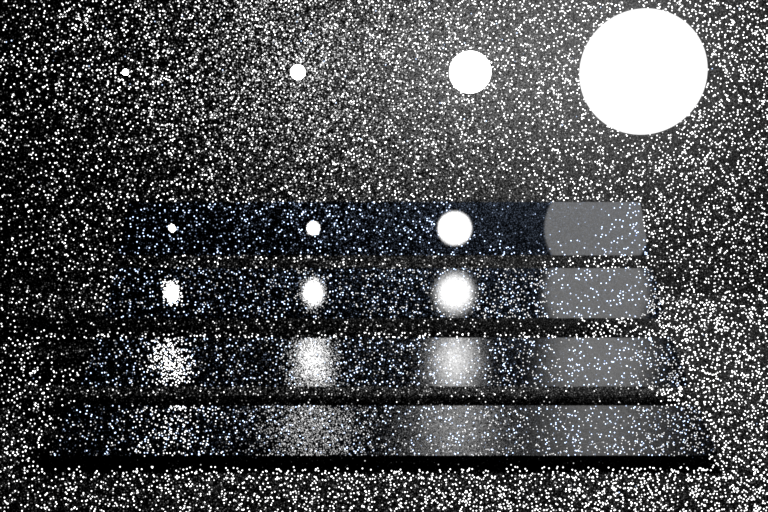
\includegraphics[width=0.52\textwidth]{bilder/veach/bsdf_64.png}
 \caption{On the upper right, where the surface is highly specular and the light sources are large, BSDF sampling performs rather well.\newline
On the lower left as well as the floor and wall, where the surface is highly diffuse and the light sources are small, BSDF sampling produces a lot of noise.}
  \label{BSDF_veach}\end{figure}



A problem with generating samples solely from the BSDF is that the path is not very likely to hit a light source. This leads to more longer paths and, when the scene is not closed, to paths completely leaving the geometry. The smaller the area covered by light sources the more paths will be leaving the scene before hitting a light source. Figure \ref{BSDFsampling_spp} shows how BSDF sampling behaves for different numbers of samples per pixel.
 
 Additional properties of BSDF sampling (as well as next event estimation) can be found in \cite{veachdiss}.


 \begin{figure}[ht!]
 \centering
 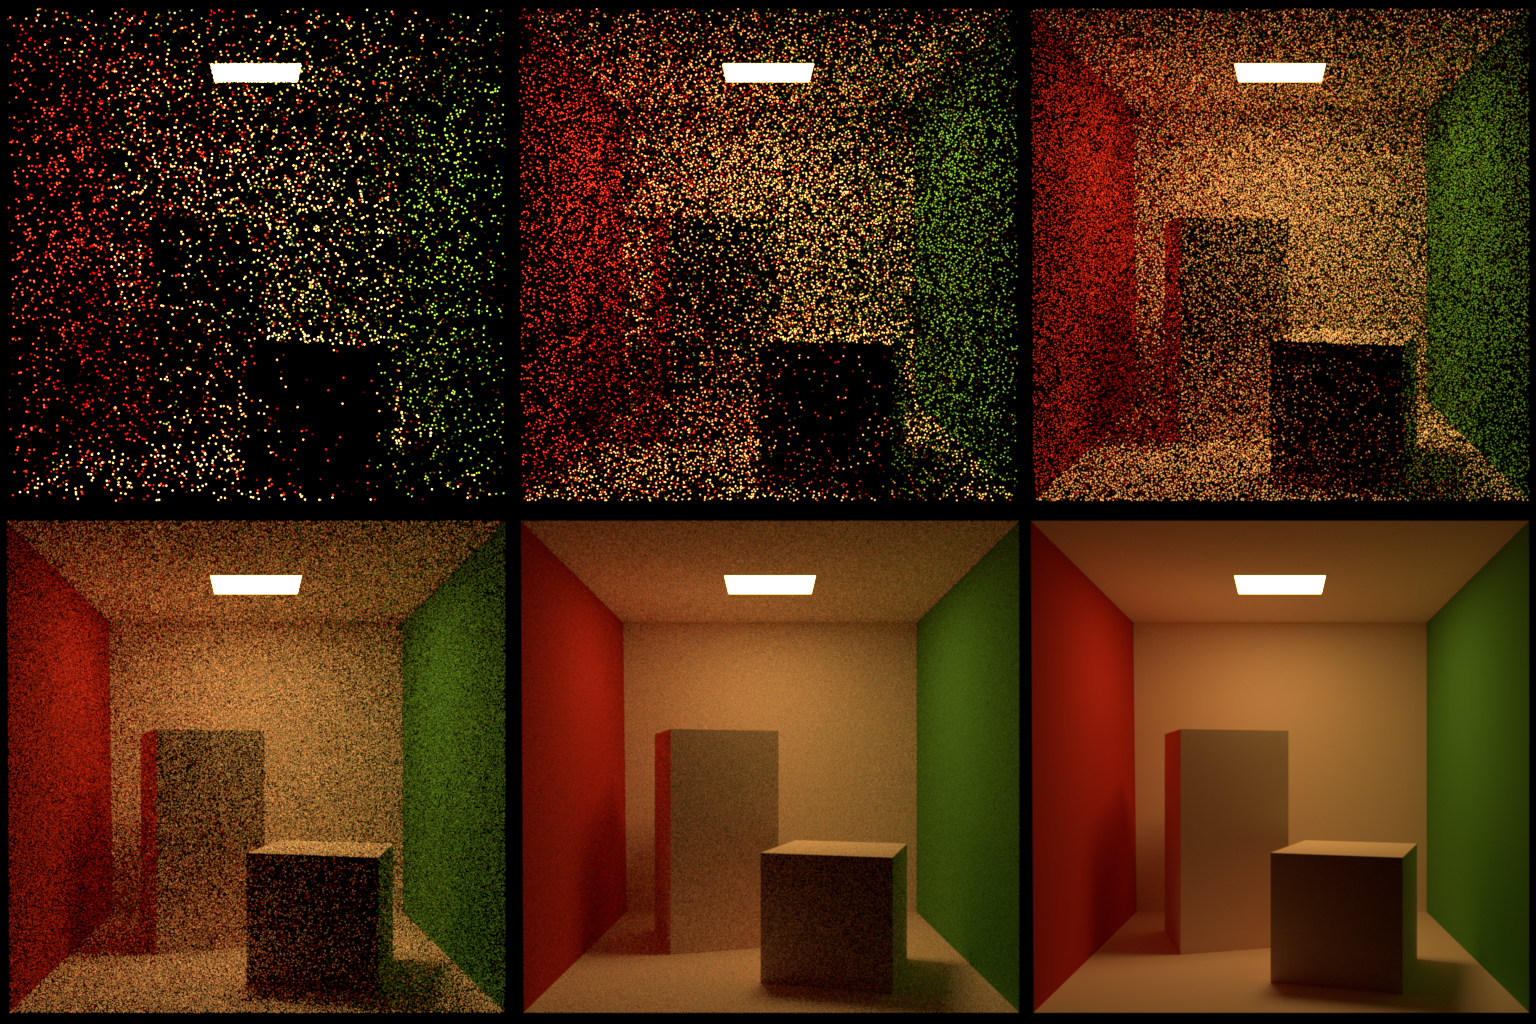
\includegraphics[width=1\textwidth]{bilder/bsdf_sampling/1-4-16-64-1024-mts.png}
 \caption{BSDF sampling with 1, 4, 16, 64 and 1024 samples per pixel, and a perfect image on the bottom right (created with another algorithm).\newline
Note how even 1024 samples per pixel still produce some noise compared to the exact solution.}
  \label{BSDFsampling_spp}\end{figure}


\subsection{Next Event Estimation}
As seen above, sampling the BSDF shows some flaws when dealing with diffuse surfaces and small light sources. Next Event Estimation (NEE) is a sampling strategy that performs by far better in these cases, but exhibits some weaknesses for specular surfaces and large light sources.\newline
With NEE, samples are not generated as outgoing directions at the surface point in order to create paths of arbitrary length, but as points on any light source instead: We take an incomplete path $(x_0,\dots,x_k)$, sample a point $x'$ on a light source and check if $x_k$ and $x'$ are visible to each other. If that's the case we have created a complete path from the camera ($x_0$) to a light source ($x'$). Since this strategy always terminates the given path, using it exclusively would result in creating mainly short paths. As a consequence NEE is usually combined with BSDF sampling.

The goal of this strategy is to use a pdf that approximates $L_i(x,\omega_i)$. Since most surface interactions attenuate the energy of incoming light, $L_i$ will presumably be a lot bigger if $\omega_i$ points directly to a light source.

In order to better understand how a pdf for NEE can be created, we look at the scattering integral over surface area. Remember the three-point form of the rendering equation \ref{tpf}, where we included a geometry term $G$ in order to compensate for the conversion from solid angle to surface area:

\begin{equation*}
L_o(x' \rightarrow x'') = \int_\mathcal{M} L(x \rightarrow x') f_s(x \rightarrow x' \rightarrow x'') G(x\leftrightarrow x')dA(x).
\end{equation*}

Now, intuitively $L(x \rightarrow x')$ will be a lot bigger whenever $x$ is actually emitting light instead of just redirecting and thereby attenuating it. As we have no analytical information on $L$ (as opposed to sampling the BSDF or cosine), we use the alternative approximation of giving a high probability to those $x$ on light sources. When combining NEE and BSDF, the multi-sample model even allows for this pdf to be $0$ for all points that are not part of a light source.

Usually a light source is picked according to its area and intensity, and a point on that light source is sampled uniformly. These probabilities are initially measured over surface area and have to be converted to solid angle, if we want to combine NEE and BSDF sampling.\\

\textbf{Strengths and Weaknesses}

As indicated above, NEE performs well for small light sources as well as highly diffuse surfaces. Veach illustrates the different aspects of NEE versus BSDF sampling with the glossy highlights problem in \cite[chapter 9.3.1]{veachdiss}. We used a replica of his scene from the Mitsuba download website \cite{mitsuba}. The results are shown in figure \ref{veach_mis} for BSDF sampling, NEE and the combination of both using the multi-sample model.\\
The biggest problem with NEE is that it completely ignores strong indirect lighting (e.g. from mirrors or glass surfaces) and can therefore not render any caustics (see figure \ref{nee_caustics}).

 \begin{figure}[ht]
 \centering
 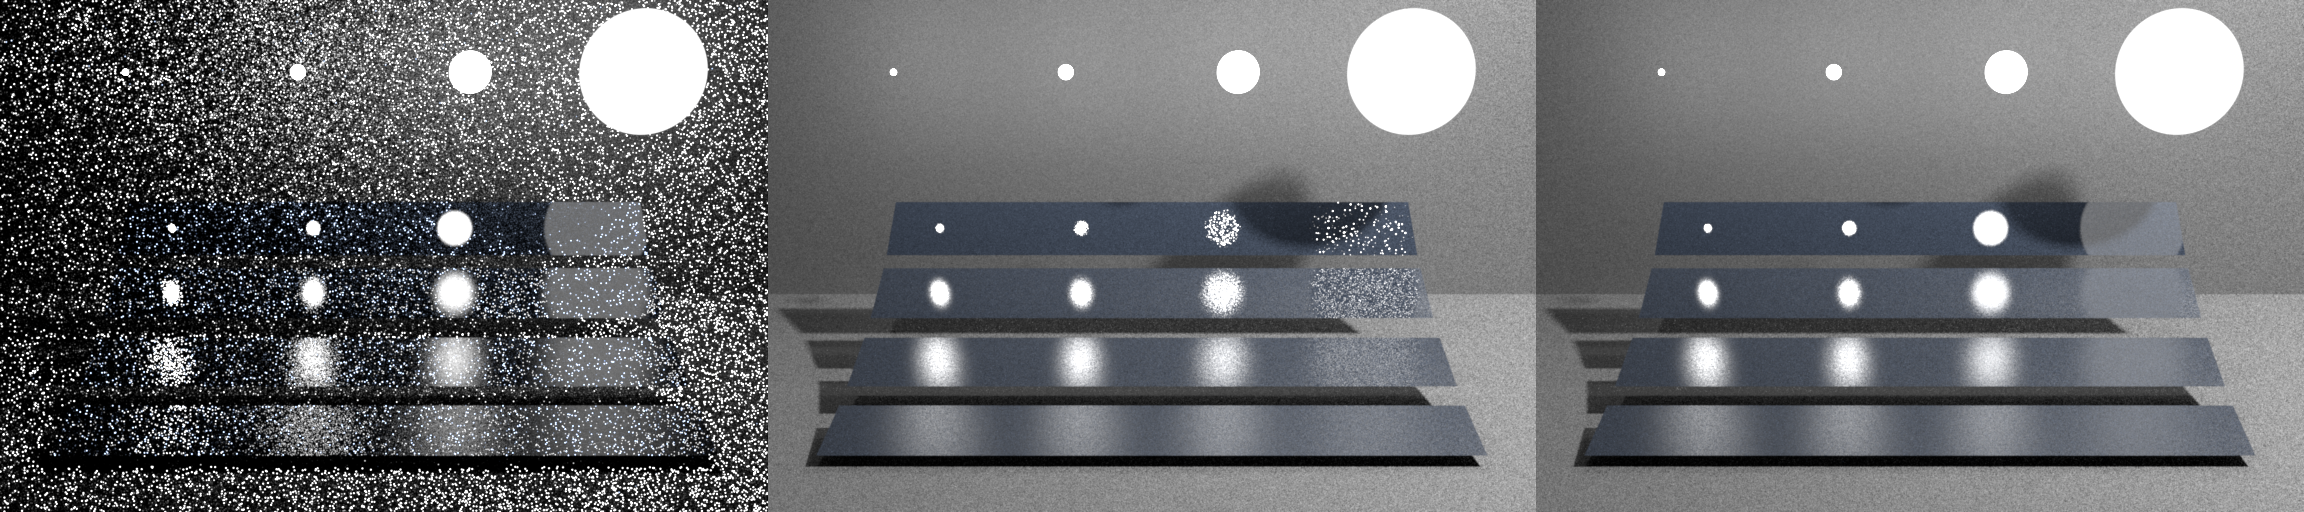
\includegraphics[width=1\textwidth]{bilder/veach/bsdf_nee_beids_64.png}
\caption{Left: BSDF sampling (good with specular surfaces and large light sources)\newline
Center: NEE (good with small light sources or diffuse surfaces)\newline
Right: MIS of BSDF sampling and NEE}
 \label{veach_mis}\end{figure}



 \begin{figure}[ht]
 \centering
 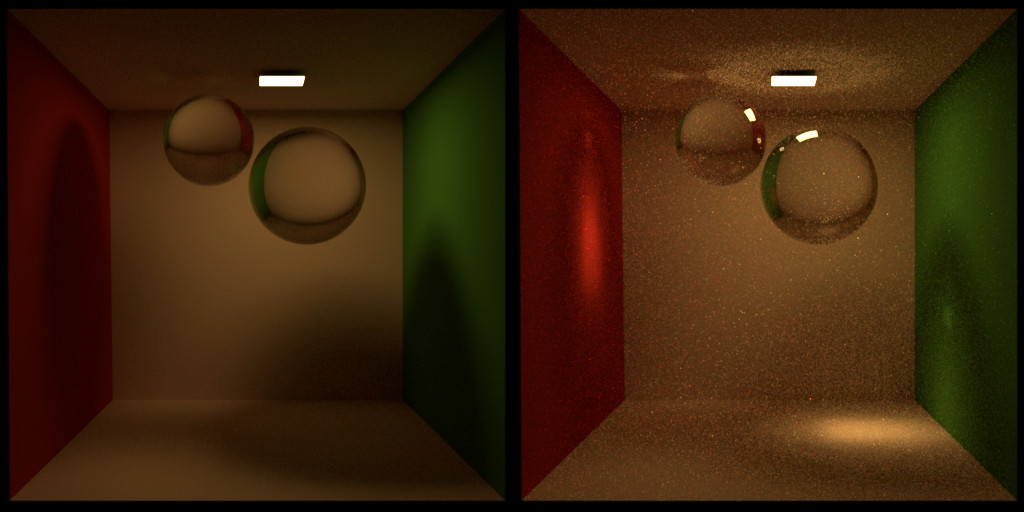
\includegraphics[width=0.8\textwidth]{bilder/kugelbox/nee_caustics.png}
\caption{Left: NEE only, the caustics are missing. Right: Reference with caustics.}
  \label{nee_caustics}\end{figure}



\subsection{Irradiance Sampling}
The main part of this thesis will cover caches for incident radiance as an alternative way to create a pdf proportional to $L_i$. While NEE only considers direct illumination and can be computed as needed, our approach to irradiance sampling requires a preprocessing step. In that step, the incident radiance - direct and indirect - is approximated and cached. Each cache is placed at a surface point $x$ and provides a pdf that is proportional to the incident radiance arriving at $x$ from different directions. The pdf values are measured over solid angle. As shown later, sampling an outgoing direction from such a cache is fast and simple, and - given certain conditions - irradiance importance sampling can offer advantages over NEE or BSDF sampling.\newline
In chapter \ref{chapter:irradiance_caching} we show how we used caches to approximate incident radiance, and chapter \ref{chapter:rendering} will explain how to use these caches for irradiance importance sampling.




\section{Path contribution}

Assuming that we have created a path $x = x_0x_1\dots x_k$ according to some strategy, we can now compute its contribution to our estimator from equation \ref{path integral estimator} as

\begin{equation*}
contribution(x) = \frac{f_j(x)}{p(x)}.
\end{equation*}

The total probability of sampling the whole path is given as the product of all probabilities used to sample a new point of the path. We only use forward sampling, meaning that we only sample new points on a path from camera to light source. Note that bidirectional techniques use both forward and backward sampling - subpaths are sampled starting both from a light source and from the camera, which affects the way their probabilities have to be computed. See \cite[chapter 10]{veachdiss} for further information.

Note that equation \ref{path integral} is measured by the area-product measure. So theoretically we have to measure our probabilities over surface area. Let $p_A(x_{i+1})$ be the probability of sampling (the direction to) $x_{i+1}$ when we are at point $x_i$, measured over surface area, and let $p_\sigma(x_i \rightarrow x_{i+1})$ be the probability of sampling $x_{i+1}$ from $x_i$ measured over solid angle. We can convert between $p_A$ and $p_\sigma$ similar to equation \ref{geotrans} as follows:

\begin{equation}
\label{pdftrans}
p_A(x_{i+1}) \cdot cos(x_i \rightarrow x_{i+1}) = G(x_i \leftrightarrow x_{i+1}) p_\sigma(x_i \rightarrow x_{i+1}),
\end{equation}

In the next equation we will replace $f_s(a \rightarrow b \rightarrow c)$ with $f_s(a,b,c)$ and $G(a \leftrightarrow b)$ with $G(a,b)$, and we will use

\begin{equation*}
W :=  \frac{W_e^j(x_1 \rightarrow x_0) G(x_0,x_1)}{p_A(x_1)}.
\end{equation*}

The total contribution of a path $x=x_0x_1\dots x_k$ from camera to light can be computed by combining $p$ and $f_j$.
\pagebreak
\begin{equation}
\label{geoweg}
\begin{split}
contribution(x) &= L_e(x_k \rightarrow x_{k-1}) \cdot W \cdot \prod _{i=1}^{k-1} \frac{f_s(x_{i+1},x_i, x_{i-1}) G(x_i, x_{i+1})}{p_A(x_{i+1})}\\
&= L_e(x_k \rightarrow x_{k-1}) \cdot W \cdot \prod _{i=1}^{k-1} \frac{f_s(x_{i+1},x_i, x_{i-1}) cos (x_i \rightarrow x_{i+1})}{p_\sigma(x_i \rightarrow x_{i+1})}.
\end{split}
\end{equation}

Equation \ref{geoweg} shows that the geometry term disappears almost completely if we measure our pdfs over solid angle. Fortunately this is also way more convenient for BSDF sampling and our caches, as these strategies only provide directions and don't make use of any information on the other surfaces in the scene - the next path point is only retrieved by casting a ray from the current path point along the sampled direction.

This also means that we can assemble the path's contribution gradually while we create it, as depicted in algorithm \ref{assembleenergy}: At each point $x_i$ we evaluate the local BSDF for the previous and sampled direction and the cosine factor for the sampled direction. We multiply these values together, and as soon as we hit a light source we multiply $L_e$ and are done.

\begin{algorithm}
\caption{Assemble a path's energy}
\label{assembleenergy}
\begin{algorithmic}
\State $weight \gets W$
\While {$x_i$ not on light source}
\State Sample $x_{i+1}$
\State $weight \gets weight \cdot \frac{f_s(x_{i+1},x_i,x_{i-1}) cos(x_i \rightarrow x_{i+1})}{p_\sigma(x_i \rightarrow x_{i+1})}$
\EndWhile
\State \textbf{return} $L_e(x_k \rightarrow x_{k-1}) \cdot weight$
\end{algorithmic}
\end{algorithm}



Note that for NEE, where we sample a point instead of a direction, a pdf measured over surface area is more convenient. So if we hit the light source deliberately by using NEE, we need to replace the last $\frac{cos(x_{k-1} \rightarrow x_k)}{p_\sigma(x_{k-1} \rightarrow x_k)}$ with $\frac{G(x_{k-1} \leftrightarrow x_k)}{p_A(x_k)}$.

\newpage
\section{The Algorithm}
\label{pathtracingalgorithm}

Algorithm \ref{weightPath_BSDF} already provided a short example of a basic path tracing algorithm that only used the BSDF to extend paths.

We will now expand that example to include BSDF sampling as well as NEE and add MIS weights according to the multi-sample model. We ignored $W_e^j(x_1 \leftrightarrow x_0)$, $p_A(x_1)$ and $G(x_1 \leftrightarrow x_0)$ in our implementation, since $W_e^j$ is usually defined in a way that all three factors are cancelled out to prevent vignetting.

We use the following notation:
\begin{itemize}
\item $p_{A,nee}(x')$ is the pdf value for sampling a point $x'$ on any light source, measured over surface area. $p_{\sigma,nee}$ is the same pdf measured over solid angle.
\item Given points $x_1, x_2$ and $x_3$, $p_{BSDF}(x_3)$ is the probability of sampling the incident direction $x_3 - x_2$ from the local BSDF at $x_2$ with outgoing direction $x_1 - x_2$.
\end{itemize}
We use the power heuristic \ref{power heuristic} to weight NEE and BSDF sampling together. A similar algorithm can be found in \cite{survey}. 

\begin{algorithm}
\caption{Path tracing with BSDF sampling and NEE}
\label{ptBSDF}
\begin{algorithmic}[1]

\State $x_0 \gets $ point on Camera
\State $\omega_1 \gets $ first ray direction

\State $x_1 \gets x_\mathcal{M}(x_0,\omega_1)$
\State $w_{BSDF} \gets 1$
\State $i \gets 1$
\State $throughput \gets 1$
\State $color \gets black$
\While {true}
\If {$L_e(x_i \rightarrow x_{i-1}) > 0$}
\State \textbf{return} $throughput  \cdot w_{BSDF} \cdot L_e(x_i \rightarrow x_{i-1}) + color$

\Else

\State
\State $x' \gets samplePointOnLightSource()$
\If {$x'$ is visible from $x_i$}
\State $w_{nee} \gets \frac{p_{\sigma,nee}(x')^2}{p_{\sigma,nee}(x')^2 + p_{BSDF}(x')^2}$
\State $L \gets L_e(x' \rightarrow x_i)$
\State $color \gets color + L \cdot throughput \cdot w_{nee} \cdot f_s(x' \rightarrow x_i \rightarrow x_{i-1}) \cdot \frac{G(x_i \leftrightarrow x')}{p_{A,nee}(x')}$

\EndIf
\State
\State $\omega_{i+1} \gets $ bsdf.sampleDirection$(x_i,\omega_i)$

\If {$ray(x_i,\omega_{i+1})$ intersects scene}
\State $x_{i+1} \gets x_\mathcal{M}(x_i,\omega_{i+1})$
\State $throughput \gets throughput \cdot f_s(x_{i+1} \rightarrow x_i \rightarrow x_{i-1})\cdot \frac{cos(x_i \rightarrow x_{i+1})}{p_{BSDF}(x_{i+1})}$
\State $w_{BSDF} \gets \frac{p_{BSDF}(x_{i+1})^2}{p_{BSDF}(x_{i+1})^2 + p_{\sigma,nee}(x_{i+1})^2}$
\Else
\State \textbf{return} $color$

\EndIf

\State $i \gets i+1$
\EndIf
\EndWhile

\end{algorithmic}
\end{algorithm}
\pagebreak


This algorithm usually creates multiple paths: One so-called ``implicit path'', where we continue to sample points from the BSDF until we accidentally hit a light source, and several ``explicit paths'' that are created by deliberately sampling a point on the light source. However, since we terminate any path as soon as it hits a light source, we always extend exactly one path. The explicit paths are terminated as soon as they are created and pose no problem in terms of an exponentially growing number of paths to pursue.






\section{Russian Roulette}
\label{chapterRussianRoulette}
In an enclosed environment, paths generated by BSDF sampling can get arbitrarily long before reaching a light source. Not only do these paths carry very little energy, they also take much more time to compute. Russian Roulette is a common solution to achieve better computing time while not manipulating the correct solution by ignoring these paths completely.

With Russian Roulette, all paths are randomly terminated after reaching a certain length: Every time before the path is extended, a random number $r$ is compared to a threshold $\alpha \in \lbrack 0,1\rbrack$. If $r>\alpha$, the path is terminated. If $r \leq \alpha$, the path is continued and weighed with $\frac{1}{\alpha}$. As a result, there will be fewer but more heavily weighted long paths and more short paths with smaller weights. As this approach still explores all possible paths it still generates a correct solution.

Too small $\alpha$ values can lead to an extremely low number of long paths, that in exchange are extremely highly weighted and result in fireflies in the final image. On the other hand, Russian Roulette will rarely cancel any paths at all, if $\alpha$ is constantly too big. Usually $\alpha$ is determined dynamically, depending on criteria such as the path's current length, its contribution or surface properties (e.g. reflectance).\\
Since very short paths will almost always be important to a pixel's color, Russian Roulette should only be applied to paths above a certain length.

However, Russian Roulette will always lead to a higher variance, so we only applied it to paths with a length over $20$.


\chapter{Caching incident radiance}
\label{chapter:irradiance_caching}
The main goal of this thesis is to approximate the irradiance across a scene using local caches. Opposed to irradiance caching (as described in chapter \ref{irradiance caching}, \cite{ward}), where all the irradiance at one point is cached in one single value, we want to cache the incident radiance for different directions.\\
This chapter will cover all relevant preprocessing steps: Choosing a cache representation, placing the caches in the scene, and filling them. The next chapter will cover the actual rendering process and describe how these caches can be used in a path tracer to importance sample the irradiance.\\
We will use the term \textbf{IRC} (incident radiance cache) to refer to a cache.

\section{Environment Map Parameterization}
\label{envmap param}
Every IRC at a certain surface point is represented by a small local environment map. Every texel of this environment map will contain the relative incident radiance around the cache's position from the direction covered by that texel.

We chose the Octahedron representation proposed by \cite{octahedronpaper}. The main advantage of this parameterization is that in comparison to cube maps and especially sphere maps, all texels cover roughly the same solid angle. Since all probabilities in our path tracing algorithm are measured over solid angles, this choice results in the least distortion when converting probabilities between texel space and solid angles. This conversion is explained in chapter \ref{solidAngleConversion}.

Plus, the conversions between directions and texels are rather simple:\\
To map a direction $d=(d_x,d_y,d_z)$ on a texel coordinate $p = (p_x,p_y)$, we first use planar projection to convert the direction vector to a point on the unit octahedron surface:

\begin{equation}
d' = \frac{d}{|d_x| + |d_y| + |d_z|}.
\label{planar_projection}
\end{equation}

Next we need to project this point on a two-dimensional texture coordinate $p$. There are several ways to do this, we chose one that yields a rectangular texture: 

\begin{equation}
p = \begin{cases}
  (d_x' - d_z' - 1, d_x' + d_z')  & \text{ } d_y' \geq 0 \\
  (d_z' - d_x'+ 1, d_x' + d_z') & \text{ } d_y' < 0.
\end{cases}
\label{planar_projection2}
\end{equation}

\begin{figure}[ht]
	\centering
\def\svgwidth{230pt}
\input{planar_projection.pdf_tex}
	\caption{Planar Projection}
\label{texture_coord}\end{figure}



Figure \ref{texture_coord} depicts the complete projection. The resulting coordinate lies in $\left[-2,2\right]\times\left[-1,1\right]$, with directions of the upper hemisphere being mapped to $\left[-2,0\right]\times\left[-1,1\right]$ and directions of the lower hemisphere being mapped to $\left[0,2\right]\times\left[-1,1\right]$. As seen in figure \ref{octamap}, texels close to $p_x = 0$ belong to similar directions on adjoint octahedron surfaces. 

\begin{figure}[ht]
	\centering
	\def\svgwidth{230pt}
  \input{octahedronmap.pdf_tex}
	\caption{The upper hemisphere is mapped to the left side, while the lower hemisphere (if needed) is mapped to the right half.\newline
The borders in the final map match the octahedron edges.}
	\label{octamap}\end{figure}


This projection is relatively easy to calculate back and forth, plus the resulting texels cover the whole area of the texture. Since both hemispheres are mapped to separate parts of the texture we can simply ignore the lower hemisphere at non-transmitting surfaces, when irradiance from below has no contribution to the outgoing light. We can then only use radiance arriving at the upper hemisphere by only using - and storing - the left half of the environment map, which also saves a considerable amount of storage space.

\section{Creating Caches}
Actually creating these caches consists of 4 steps: Photon Mapping, distributing the positions of the caches over the scene, filling the caches and storing them.\\
Since we intend to fill the caches with incident radiance, we need some way to approximate it. We do this with a modified version of photon mapping. When the photon mapping is done, the photons are used to place and fill the caches.



\subsection{Modified Photon Mapping}
\label{modified photon mapping}
The idea of photon mapping is to trace a huge number of emitted photons from all light sources along their paths and store a photon at every surface point along that path. Originally, the resulting photon map would then be used to render the image. We give a short introduction on photon mapping as a stand-alone rendering technique in chapter \ref{photon mapping}.

\newpage
\textbf{Creating a photon path}

A photon path is initialized by sampling a point and outgoing direction for a photon and then tracking it across the scene. Whenever there are multiple light sources, a light source $L$ is chosen with a probability $p_L$ proportional to its surface area $A_L$ and its flux $\Phi_L$: 

\begin{equation}
p_L = \frac{A_L \cdot \Phi_L}{\sum_{L'}A_{L'} \cdot \Phi_{L'}}.
\end{equation}

For simplicity's sake we only consider area light sources here. A point $x$ on light source $L$ is sampled uniformly with probability $p_x = 1/A_L$, the probability for sampling direction $\omega_o$ at this point is $p_\omega$. Given a light source L, let $L_e(x,\omega_o)$ be the power of that light source for the given origin $x$ and direction $\omega_o$. When $N$ photons are emitted, the initial energy of the photon emitted from light source $L$ at $x$ into $\omega_o$ is given as

\begin{equation}
\label{initialenergy}
\frac{L_e(x,\omega_o)}{p_L \cdot p_x \cdot p_\omega \cdot N} =  \frac{L_e(x,\omega_o)}{p_\omega} \cdot \frac{\sum_{L'} A_{L'} \Phi_{L'}}{\Phi_L \cdot N}.
\end{equation}


This photon is then traced across the scene. Whenever the photon's path intersects a diffuse surface, a photon with the current energy is stored. At any intersection $y$, no matter if it's diffuse or specular, the outgoing direction $\omega_o$ of the photon path is sampled from the surface's adjoint (see \ref{BSDF}) BSDF and the incoming direction $\omega_i$. The path is continued into the sampled direction and the energy is weighed with the BSDF's value $f_s(\omega_i,y,\omega_o)$ divided by the probability of sampling $\omega_o$.\\

\textbf{Adjustments for IRCs}

Since we plan to use photon mapping to approximate incident radiance instead of rendering an image we need to make some adjustments to this process. One of them are the stored photons themselves: Each of our photons consists of its position including the local surface coordinate system, its incoming direction, a pointer to the surface's BSDF and its energy. The next section will explain why the local coordinate system is necessary. The BSDF is needed in case we want to place a cache at the photon's position: It tells us whether we need an environment map for both hemispheres or only one. We don't need the actual energy distribution over different wavelengths; storing a photon's average energy in a single float value is sufficient.

Besides, we only need the relative incident radiance from all directions to create a cache. This allows us to ignore the constant factors in \ref{initialenergy} (the fraction on the right) when computing a photon's initial energy; we can use 

\begin{equation}
\frac{L_e(x,\omega_o)}{p_{\omega}}
\end{equation}
 
 instead. To avoid unnecessary computing, we cancel photon paths when their accumulated energy falls too close to zero, when the path length reaches 32 and using Russian Roulette. As soon as all photon paths are complete, all created photons are stored in a k-d tree (\cite{kdref1}, \cite{nanoflann}).


\newpage

\subsection{Placing Caches}
\label{placing caches}
There are two interesting areas for placing IRCs: Those with much incident light, and those that are potentially hit very often when using path tracing later on.

To cover the latter, we send a camera ray through the upper left corner in every $8\times 8$ pixel block. If the BSDF at its first intersection with the scene is smooth, we place a cache at that position. Otherwise the ray will be traced until it leaves the scene or until a surface with a smooth BSDF is hit so we can place a cache. We call the resulting caches \emph{camera caches}.

The remaining cache positions are adopted from the first $n$ photon positions from the photon mapping step. This will lead to many caches in areas where many photons arrive, and place less caches in areas where only few photons intersect the scene.  Since the photon paths were constructed randomly,  the distribution of cache positions generated from simply taking the first $n$ photons will  be similar (on average) to choosing the photons randomly.

Note that from now on we have almost no information concerning the surface properties (BSDF, geometry, normals) at the cache position. We only know the positions themselves and that they are placed at non-delta BSDFs. To avoid inconsistent coordinates later on, it is necessary to give each cache its local coordinate system. Luckily we already stored these systems with every photon and can simply use these for the photon caches. The camera caches get their coordinate system from the intersection information which is still available when the caches are placed in the scene.

At this point we also need to decide whether to create a cache for irradiance from both hemispheres or only one. To do so, we look at the BSDF (which is either stored in the photon or can be retrieved from the intersection information for camera caches): If it is transmitting, we create an empty environment map for both hemispheres and store it at the position with its coordinate system. Otherwise a map for the upper hemisphere is created and stored. Practically the only difference between these two IRCs is the length of the array containing the environment map's texels. We don't consider materials where only irradiance from below contributes to radiance leaving at the upper side.

\subsection{Filling a Cache}
After the caches are created and placed across the scene we need to fill them with an approximation of the incident radiance around them. The number $k$ of photons used to fill a cache is fix and can be adjusted before the image is rendered. Filling a cache works like this:
\newline
\begin{algorithmic}
\State $photon list \gets $ \Call{$kdTreePhotons.getKClosestPhotons$}{$k,cache.position$}
\ForAll{$Photon$ $p$ in $photon list$} 
	\State $incoming\_direction\_local \gets $\Call{$cache.transformToLocal$}{$p.direction$}
    \If {$cos(local\_incoming\_direction) > 0$ $||$ $cache\_for\_both\_hemispheres$}
        \State $texel \gets $ \Call{$cache.convertDirectionToTexel$}{$incoming\_direction\_local$}
        \State $cache.environmentMap\lbrack texel \rbrack += p.energy$
    \EndIf
\EndFor
\end{algorithmic}

Whenever a photon is deemed useful to fill a cache, its incoming direction is converted to a texture coordinate for our octahedron environment map (see equations \ref{planar_projection} and \ref{texture_coord}).

We found that filtering the caches considerably reduces the noise in the final image.
First we apply bilinear filtering to distribute the energy of each photon over the texel itself and its left/right, upper/lower and diagonal neighbour. This is done while the photons are added to the cache one by one.

After the cache has been filled, we use a Gaussian filter

\begin{equation*}
\frac{1}{16}\begin{pmatrix} 1 & 2 & 1 \\ 2 & 4 & 2 \\ 1 & 2 & 1 \end{pmatrix}
\end{equation*}

on all texels. In order to filter the texels on the edge, we simply added the texels from the opposite side. Theoretically, this is not correct, as texels on opposing edges may correspond to opposing directions (see figure \ref{octamap}). But the improvement on the images was big enough, so we stayed with that simplification.\\
We found that Gaussian filters showed a bigger improvement than bilinear filtering, and the combination of both could noticeably reduce the noise of an image, see figure \ref{filtervergleich}.\\

\begin{figure}[ht]
	\centering
  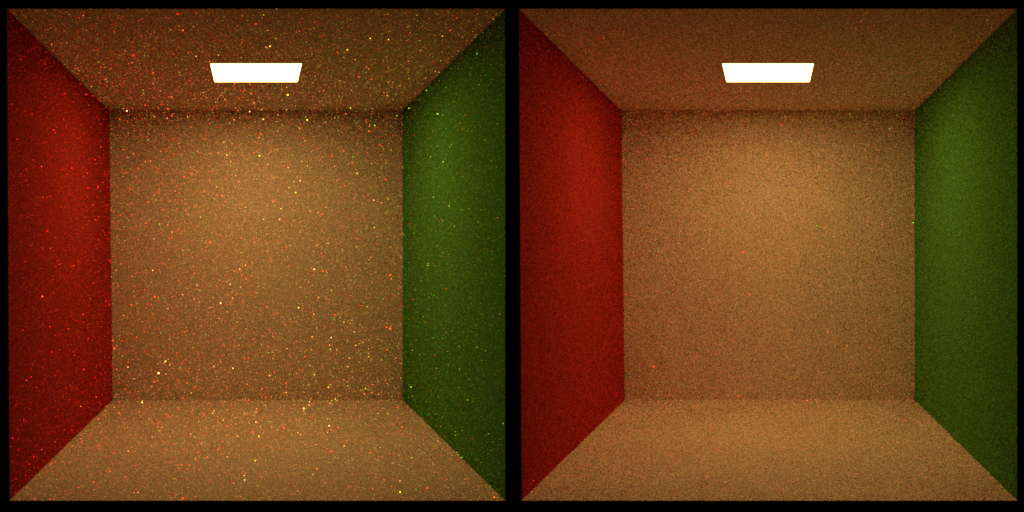
\includegraphics[width=1\textwidth]{bilder/filter/filtervergleich.png}
	\caption{Left: No filtering.\newline
Right: bilinear filtering and Gaussian filter.\newline
Both images were rendered with IRCs only (no BSDF sampling or NEE), using 150.000 photon paths ($\approx$ 750.000 photons), 20.000 caches, 500 photons per cache and 64 samples per pixel.}
	\label{filtervergleich}
\end{figure}



 We also tried to weight the energy contribution of a photon with its distance to the cache's position or with the Epanechnikov kernel \cite[chapter 8]{epanechnikov}. The difference was barely noticeable, but the images seemed a little better without these weights.

One last thing to note is that the number of photons actually contributing to a cache may be lower than $k$. Figure \ref{fill_cache_cos} illustrates an example.

\begin{figure}[ht]
	\centering
\def\svgwidth{250pt}
  \input{bilder/fill_cache_cos.pdf_tex}
	\caption{When filling the cache with 4 photons, photons p1 to p4 are considered and p5 is ignored. However, the incoming direction of p2 results in a negative cosine with the cache's surface normal, meaning that the photon arrives from below from the cache's point of view. Thus p2 is discarded for this cache and only p1, p3 and p4 are used to fill it.}
	\label{fill_cache_cos}
\end{figure}


\newpage
\subsubsection{Creating a useful probability density function}
The next step is to convert the filled environment map to a probability density function that can be used to sample an outgoing direction proportional to the incident radiance during path tracing. The main idea is to normalize the sum of all texels of the environment map to 1 and then sample directions according to the probability values stored in the texels. Obviously, the first step towards a useful pdf is simply that: add up all energy values from the environment map and divide every texel's value by that sum.

However, we have to consider that Monte Carlo integration requires the pdf to be greater than zero wherever the integrated function contributes to the integral. So we have to make sure that our pdf isn't equal to 0 when radiance arriving from the corresponding direction can contribute to the integral. With non-delta BSDFs that is the case for all directions (in the upper hemisphere), so we have to set all texels with value 0 to a bigger value. This value should be big enough so it won't cause any floating point precision problems - either by being ignored completely in the final pdf or by causing fireflies due to dividing by very small numbers. On the other hand the value should not affect the quality of the radiance approximation stored in non-zero texels.

We tried several options: The first one was setting the zeros to the smallest positive value from all other texels before normalizing. However, in many cases this value turned out to be too close to zero and disappeared completely after the normalization. Even normalizing, setting all 0 texels to the smallest value after normalizing, and normalizing again resulted in near-zero values that didn't work well in the final image.\newline
Next we tried setting every value below half average of all non-zero values to half average. The reason for that idea was that many caches had some texels with values around some 100, but a lot more texels containing positive values below 1. This approach caused by far the most noise in the final image.\newline
After looking at several normalized environment maps, we tried to simply set all values smaller than 0.0002 to 0.0002 and normalize again. This seemed to be working quite well so far. We even tried combining this approach with the first one, but as it turned out the minimal value was always smaller than 0.0002, regardless of whether it was picked before or after the first normalization. Different thresholds from 0.0001 to 0.001 didn't produce any noticeable differences in the final images.

There's also a reason not to set every 0 to a fix non-zero value before the first normalization: The sums of two caches can easily differ in an order of 2 magnitudes. So while setting all 0 texels to, say, 1 may work perfectly fine for one cache with a (previous) sum of some 100, it can totally destroy the irradiance approximation for another one with a sum of 50 or just disappear again for caches in bright regions with sums up to some 1000. Additionally, the initial sum of a cache depends on the number of photons used to fill it and the overall energy of these photons, while the average value of a texel also depends on the resolution of the octahedron map. Considering all these uncertainties it seems more reasonable to increase the 0-texels after a first normalization, when we can make a more precise statement about the overall properties of the cache.

The values of the environment map now form a valid probability density function that can be used to sample directions. This pdf is currently measured over the texel space, where each texel covers a unit square and all texel values sum up to 1.\\
To improve computation time we also create a second environment map (the $cdf\_map$) containing the cumulative density function for that pdf and added it to the cache. See chapter \ref{path extension} on how samples are torn from these environment maps.

\newpage
\subsubsection{Convert probabilities to solid angle}
\label{solidAngleConversion}
Generating samples is not the only purpose of these caches. The other one is to get the probability linked to the sampled direction, and to compute the probability of sampling a given direction from a cache. These probabilities are needed to compute weights for Multiple Importance Sampling and to compute the probability of sampling a path.\\
While probabilities for path tracing are usually measured over solid angle, our pdf is measured over a rectangle (or square in case only the upper hemisphere is important). Its width and height correspond to the number of columns and rows of the environment map, and each texel covers the area of one unit square. Remember that the pdf values were normalized to sum up to one.

Unfortunately, there is no easy way to analytically compute the solid angle covered by each unit square in our environment map. Ignoring this problem and directly using the probability value from a cache resulted in almost completely white images. This is due to the fact that with a $16\times 16$ resolution, every pdf value is roughly $\frac{2\pi}{256}$ times as big as it should be. Thus the accumulated probability of sampling a certain path is several orders of magnitude smaller than the correct value, and dividing by it causes the energy to reach insanely high values.\newline
Approximating the solid angle measure by multiplying with $\frac{size\_of\_environmentmap}{2\pi}$ isn't enough either: The overall energy of the resulting images seemed about right, but it was rather weirdly distributed (see figure \ref{solid_angle_korrektur}). So we created another map to approximate the solid angle covered by each texel:
\newline
\begin{algorithmic}
\State $solid\_angle\_map \gets $new $octahedronMap$ \Comment upper hemisphere only
\State $numSamples \gets 1000 \cdot solid\_angle\_map.width \cdot solid\_angle\_map.height$
\For{$i = 0$ to $numSamples$}
	\State Vector3 $sample \gets $ $createRandomSampleOnHemisphere()$
	\State Vector2 $texel \gets $\Call{$solid\_angle\_map.convertDirectionToTextureCoordinate$}{$sample$}
	\State $index \gets \lfloor texel.x \rfloor + solid\_angle\_map.width ^* \lfloor texel.y \rfloor$
	\State $solid\_angle\_map\lbrack index \rbrack \gets solid\_angle\_map\lbrack index \rbrack + 1$
\EndFor
\For{($i=0$ to $solid\_angle\_map.length$)}
	\State $solid\_angle\_map\lbrack i \rbrack$ $/=numSamples$ \Comment normalize to 1
	\State $solid\_angle\_map\lbrack i \rbrack$ $^*= 2\pi$ \Comment integral over one hemisphere is $2\pi$
\EndFor
\end{algorithmic}

At the end every texel represents the relative solid angle covered by its area. Central texels and those close to the border represent directions close to the surface's normal and along the surface itself respectively and will hold smaller values. The areas in the middle of each octahedron surface are close to parallel to the unit hemisphere and thus cover a bigger solid angle. Figure \ref{solid_angle_map} shows the resulting maps for $4\times 4$, $8\times 8$ and $16\times 16$ texels, and figure \ref{solid_angle_skizze} depicts the relation between texel area and solid angle.

\begin{figure}[ht]
	\centering
  
\includegraphics[width=0.8\textwidth]{bilder/solid_angle_maps.png}
	\caption{Solid angle maps with $4\times 4$, $8\times 8$ and $16\times 16$ texels for one hemisphere}
	\label{solid_angle_map}
\end{figure}

\begin{figure}[ht]
\centering
\def\svgwidth{200pt}
\input{bilder/solid_angle_skizze.pdf_tex}
\caption{Solid angle areas covered by texels of different height for a 8x8 map. Texels on the octahedron surface's center (blue, green) cover a larger solid angle than those close to the surface (yellow) or at the top (red).\newline
Note that the difference between the texel values also depends on their horizontal distribution.}
\label{solid_angle_skizze}
\end{figure}

A pdf value from a texel in a cache's environment map can now be converted to a probability value measured over solid angle by dividing it by the value from the corresponding texel in the solid angle map. This can be done for all texels in all environment maps in a preprocessing step, as the number of accesses to caches during the actual rendering may easily exceed the total number of texels. \newline
The solid angle map can also be doubled and then applied to the lower hemisphere. In that case its values will sum up to $4\pi$, which equals the integral over the unit sphere.

\begin{figure}[h!]
	\centering
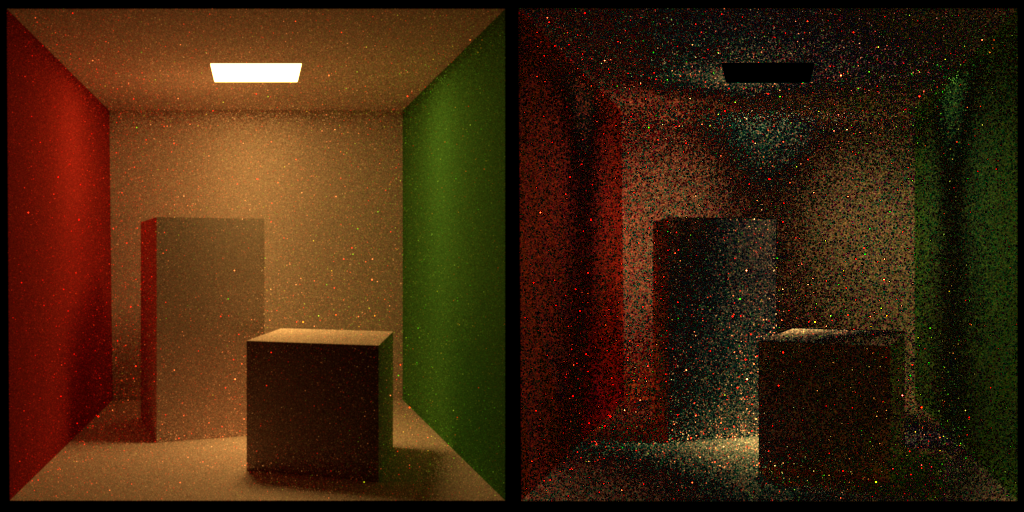
\includegraphics[width=1\textwidth]{bilder/solid_angle_difference.png}
\caption{Left: Solid angle correction with $\frac{width \cdot height}{2\pi}$\newline
Right: Difference with correct reference, multiplied by $4$. Note the vertical stripes on the wall in both images and the bright area in the middle of the floor.}
\label{solid_angle_korrektur}
\end{figure}

\clearpage
\subsection{Storing Cache}
\label{storing cache}
All caches are stored in a k-d tree (\cite{kdref1}, \cite{nanoflann}) for fast and easy access. The k-d tree containing the photons won't be needed again and can be deleted.
In the end, each IRC consists of the following components:
\begin{itemize}
\item An octahedron environment map containing the probability density function, measured over solid angle, that approximates the incident radiance around the cache. We will call this one the $pdf\_map$.
\item An additional map containing the cumulative density function for faster sampling, called $cdf\_map$. Note that the cdf is created after the last normalization, but before the pdf is adapted to the solid angle measure.
\item Its position.
\item Its local coordinate system.
\end{itemize}

\chapter{Rendering}
\label{chapter:rendering}
This chapter will describe how the IRCs from the previous chapter can be used to improve path tracing.
We will use the terms "'BSDF sampling"' and "IRC sampling"' for the process of sampling an incident direction and its probability from a surface point's BSDF or corresponding IRC respectively. How samples can be generated from a BSDF will not be discussed here any further.\newline
The first part of this chapter will cover generating samples and probabilities from an IRC. The second part combines IRC sampling with BSDF sampling or NEE using Multiple Importance Sampling. In the end we evaluate the results.


\section{Sampling Caches}
\subsection{Path Extension}
\label{path extension}
As described in chapter \ref{chaper:PathTracing}, path tracing creates random paths starting at the camera and traces these paths across the scene until either a light source is hit or the path leaves the geometry. To do that, we need to choose a new direction every time the path hits a surface at an intersection point $x$. This is normally done by sampling an outgoing direction from the surface's BSDF. In that case the applied pdf is proportional to the BSDF term from the rendering equation. The goal of our IRCs is to use a pdf which approximates the incident radiance $L_i(\omega_i,x)$ instead of the BSDF.

Our basic algorithm for sampling a new outgoing direction proportional to the irradiance consists of several steps: Picking an appropriate cache, sampling a direction and computing its probability.\\
So, first we have to choose the cache we want to use. Sometimes, especially at corners, thin walls or curved surfaces, the closest cache can have another normal than the surface at $x$ itself. If the deviation is small enough, the cache can be used anyway. However, if the cache's rotation is too severe, it might be better to pick one of the next closest caches more parallel to the surface at $x$. We chose $0.9$ to be the threshold for the cosine between the cache's and surface's normal and never considered more than the 5 closest caches.\newline
This may seem arbitrary, but in our example scenes most caches violating that threshold had a cosine of $0$ or less to the surface. Plus whenever a cosine was positive but below 0.9, some of the other closest caches often exhibited bigger values. We also didn't experience any problems with spheres, since the caches were always placed densely enough.

With more complex scenes and small spheres in rarely lit areas that are not seen by the camera directly but hit many times for indirect lighting, one would have to test if 0.9 is still a good choice or if a smaller values would be a better option. On the other hand, if only few photons arrive in a region in the first place, it might prove more useful to just use normal BSDF sampling there.

Instead of always choosing the closest cache (or that one of the 5 closest ones with the best cosine), we decided to randomly pick one of those caches that was among the 5 closest to $x$ and also had the best cosine value. In most cases these were all 5 closest caches with a cosine of 1. This process is depicted in algorithm \ref{algopickcache}.\newline

\begin{algorithm}
\caption{Pick Cache}\label{pickCache}
\begin{algorithmic}[1]
\Procedure{pickCache}{$surfacePoint$}
\State $cacheList \gets kdTreeCaches.getKClosestCaches(5,surfacePoint.position)$
\State $bestCos \gets -1$
\For {$i=0$ to $4$}
\State $currentCache \gets cacheList\lbrack i\rbrack$
\State $currentCos \gets cos(currentCache.normal, surfacePoint.normal)$
\If{$currentCos > bestCos$} 
\State $bestCos\gets currentCos$
\State $bestCache \gets currentCache$
\ElsIf {$currentCos == bestCos$ $\wedge$ $getRandomNumber() > 0.6$}
\State $bestCache\gets currentCache$
\Else
\EndIf
\EndFor
\If {$bestCos > 0.9$}
\State \textbf{return} $bestCache$
\EndIf
\State \textbf{return} $null$ \Comment {sample BSDF instead}
\EndProcedure
\end{algorithmic}
\label{algopickcache}
\end{algorithm}


Line $7$ ensures that we only use caches with the highest cosine value. Line $10$ takes care that we pick one of the best caches at randon, with closer caches having a higher probability of being chosen. If all five closest caches are rotated too much towards the surface at $x$, we resort to BSDF sampling just this once.

As it turns out, choosing between the 5 closest caches instead of just using the closest cache (if its cosine is high enough) consumes a third of the total computation time \ref{durations}. Plus we could not see any difference in the resulting images as long as enough IRCs were available. Maybe picking one of 5 caches is more useful for more complex scenes than our simple examples, where there is more curved geometry or edges.

After a cache is chosen, the next step is sampling a direction from that cache. For that purpose three random numbers between 0 and 1 are required. The first one is used to pick a texel from the cache's environment map. To do that we look for the field in the cache's $cdf\_map$ (see chapter \ref{storing cache}) with a value bigger or equal to the random number. The other two are needed to sample a point within the texel. This point is converted to a direction (reverse equations \ref{planar_projection} and \ref{planar_projection2}).

As we always need the probability of the sampled direction whenever a direction is sampled, algorithm \ref{sampleCache} also returns the probability for sampling the direction. Note that while the cdf was created from a pdf that sums up to one, the returned probability is measured over solid angle and was computed after the cdf was created.\newpage


\begin{algorithm}
\caption{Sample Direction from Cache}\label{sampleCache}
\begin{algorithmic}[1]
\Procedure{sampleDirection}{$cache,pdfValue,rand1,rand2,rand3$}
\State $texel\_index \gets $ \Call{binarySearch}{$cache.cdf,rand1$}
\State $pdfValue \gets cache.pdf\_map\lbrack texel\_index\rbrack$
\State $texel.x \gets texel\_index \% cache.mapWidth + rand2$
\State $texel.y \gets texel\_index / cache.mapWidth + rand3$
\State $Vector3D$ $direction \gets cache.texelToDirection(texel)$
\State $direction \gets cache.coordinateSystem.toWorld(direction)$
\State \textbf{return} $direction$
\EndProcedure
\end{algorithmic}
\end{algorithm}


We use binary search to find the index of the sampled texel in our $cdf\_map$ more efficiently. This index yields the probability for its texel from the $pdf\_map$, we write that probability to $pdfValue$ so it can be used later on. \\
Note that the pdf is designed for texels with an area of $1\times 1$, so we can get a random point within that texel from lines $4$ and $5$. Line $6$ converts this point to a point in $\lbrack -2,2\rbrack \times \lbrack -1,1\rbrack$ (or $\lbrack -2,0 \rbrack \times \lbrack -1,1\rbrack$, see chapter \ref{envmap param}) and then to a direction in local coordinates (the upper axis matches the top of the octahedron), which is converted to a direction in global coordinates in line $7$.


After a (global) direction $\omega$ is sampled, we can continue the path along $\omega$. The last thing left to do is to weight the energy carried along the path. Therefor we have to evaluate the BSDF at $x$ with $\omega$ as incoming (!) direction $\omega_i$ and appoint the direction where the path came from as outgoing direction $\omega_o$. The energy carried along the path can be weighted just as in algorithm \ref{assembleenergy} according to equation \ref{geoweg} as follows:\\

\begin{algorithm}
\caption{Weight path energy for Monte Carlo integration}
\label{weight1}
\begin{algorithmic}
\State $bsdfValue \gets x.bsdf.eval(\omega_i,x,\omega_o)$
\State $cos \gets cos(\omega_i,x.normal)$
\State $pathEnergy \gets pathEnergy \cdot bsdfValue \cdot cos / pdfValue$
\end{algorithmic}
\end{algorithm}

Note that the BSDF technically evaluates directions represented in local coordinates at $x$, so we would actually have to convert the directions from world to local coordinates first. Fortunately, if the cosine of the used cache happens to be $1$, we can skip the transformation of $\omega_i$ and just use the local cache coordinates from line 6 in algorithm \ref{algopickcache} instead, as long as the rendering framework can guarantee consistency of both coordinate systems.

However, there are cases when IRC sampling is not a good option: At specular surfaces, only light from one direction (or two for transmitting materials) actually contributes to the integral to compute. It is therefore unnecessary to randomly sample several directions, we can directly sample the one (or 2) important direction from the surface's BSDF. Note that in chapter \ref{placing caches} we only placed caches at non-specular surfaces: The cache positions were created either from photons (which are only stored for non-delta BSDFs) or from camera rays (which were traced across the scene until a surface with a non-delta BSDF was found).\newline
It might also happen that there are no caches nearby, or that the closest caches are rotated too much to provide useful information. In these cases we fall back on conventional BSDF sampling. 




\newpage
\subsection{Computing probabilities for given directions}
\label{computePdf}
For simple path tracing with implicit paths from IRC sampling only, the previous section contains all the steps we need. However, if we want to combine IRC sampling with NEE or BSDF sampling, we also need to be able to extract a probability value from a cache for a given direction in order to compute MIS weights.\newline
Therefor we first pick a cache just like in algorithm \ref{pickCache}. Next we convert the direction to local coordinates in the cache's coordinate system and then on to texture coordinates according to equations \ref{planar_projection} and \ref{planar_projection2}. A simple access to the cache's $pdf\_map$ at the computed texel yields the probability for having sampled the given direction with this cache, measured over solid angle.









\newpage
\section{Combining BSDFs and Caches}
\label{combining BSDFs and caches}
The figures in chapter \ref{importance_sampling_options} showed the flaws of choosing only one local sampling method. Figure \ref{veach_mis} already compared BSDF sampling and NEE. And while our IRCs are capable of rendering caustics, they also produce a considerable amount of noise. This noise can be worse or better than the noise we get from sampling the BSDF, depending on the scene and the quality of the caches.\\
As opposed to combining BSDF sampling and NEE, BSDF and IRC sampling cannot be done at the same time: Since we use path tracing, we don't want to split up a path into two paths whenever we hit a surface. Hence we need a way to choose between BSDF and IRC sampling and a way to combine them.

We use the BSDF's roughness to decide whether to sample the BSDF or IRCs. If the BSDF is ideally diffuse, the BSDF itself will have the same value for every direction and we cannot gain much information or increase the integrand by sampling the BSDF. On the other hand, if we hit a (near) delta BSDF, for most of the directions the incident radiance will have (almost) no contribution due to the BSDF being close to zero for most angles.

There are certain reasons not to importance sample for irradiance at all. One are delta-BSDFs: Whenever a surface is perfect specular, perfect transmitting or both, there is only one (or two) directions that actually contribute light to the current path. Whenever we hit a surface with a delta-BSDF, we will automatically only sample the BSDF with MIS weight 1, and also skip the next event estimation (if included) completely, since the probability of it having any contribution at all is zero.

Another case depends on the placement of the caches. Sometimes there might just be no caches available close to the current surface point. In simple scenes, this is almost never the case, but we can never be sure to prevent this completely, especially with more complex scene geometry.\newline
A similar case is a more complex, curved geometry. For example, consider placing caches on a sphere. Since we can never cover the whole surface area of a sphere with points, there will always be points that are hit by camera rays but have no cache at their exact position. There might be a cache very close to them, but judging from an analytical point of view the angle between their normals will never be 0. If that angle is still small (or the cosine between them big) enough, we can ignore the deviation and still use the cache, for everything we have was only approximated in the first place. We allowed a small margin of difference between the cache's normal and the surface point's normal (see \ref{path extension}). But whenever the cosine is smaller than 0.9 we ignore the caches and sample the BSDF with weight 1.\newline
If the cosine of the selected cache is bigger than 0.9 but less than 1, the outgoing direction of our path can be sampled from the IRC. It will however be converted to global and then to local coordinates at the intersection point in order to evaluate the BSDF at that point. Note that the sampled drection was represented in local cache coordinates at first and would also have been converted to global coordinates for a cosine of 1 anyway. See algorithm \ref{pickCache} on how caches are picked depending on their cosine to the surface normal at the current intersection point.




\subsection{Multiple Importance Sampling of BSDFs and IRCs}
\label{mis_BSDF_irc}
As implied in the previous segment, we will only actually combine BSDF and IRC sampling whenever we hit a surface with a non-delta BSDF and if a cache with a good enough cosine to the surface normal is near. In all other cases we continue our path by generating a sample from the BSDF with MIS weight 1.\newline
In this section we show how we decided on a probability to select either BSDF or IRC sampling, and how to compute the MIS weights for each of them.

The Mitsuba Renderer, which was used as a framework to implement this work, offers the roughness of a BSDF in the form of a floating point value $\in\lbrack 0,1\rbrack$. A roughness value of $\infty$ is used in addition to indicate perfectly diffuse surfaces.\newline
We decided that even if a surface is completely diffuse, BSDF sampling should not be ignored completely. Then again we never want to pick IRC sampling at perfectly specular surfaces for reasons explained above. So we decided on $\alpha = min($roughness$,0.9)$ as a threshold for randomly selecting BSDF or IRC sampling.

Chapter \ref{multiple importance sampling} explained how $n$ exclusive sampling techniques can be combined with the one-sample model. In our case BSDF sampling is chosen with probability $1 - \alpha$ and IRC sampling with probability $\alpha$. These probabilities obviously sum to one, they match $c_1$ and $c_2$ in equation \ref{onesample}.\newline
Assume we generated a random number $>\alpha$ and sampled some direction $\omega$ with a probability $p_{bsdf}$ from the BSDF. To compute that sample's MIS weight we also need to compute the probability $p_{cache}$ for having sampled $\omega$ from the chosen cache (see chapter \ref{computePdf}). With both pdfs being measured over solid angle, the weighting function $w_{bsdf}$ for the sampled direction can now be determined by the balance heuristic:

\begin{equation*}
w_{bsdf} = \frac{p_{bsdf}}{p_{bsdf}+p_{cache}}.
\end{equation*}

According to equations \ref{onesample} and \ref{geoweg} the total weight we have to multiply to the energy carried along the path is

\begin{equation*}
pathEnergy ^*= \frac{w_{bsdf}}{(1-\alpha)} \cdot \frac{f_s \cdot cos(\omega)}{p_{bsdf}}.
\end{equation*}

Assuming that the path's energy was already weighted similar to algorithm \ref{weight1} with $p_{bsdf}$ as $pdfValue$ before, we can weight the path energy like this: \newline

\begin{algorithmic}
\State $totalWeight \gets \frac{p_{bsdf}}{(1-\alpha) \cdot (p_{bsdf}+p_{cache})}$
\State $pathEnergy \gets pathEnergy \cdot totalWeight$
\end{algorithmic}


If the initial random number was $\leq \alpha$ and \ref{weight1} was already executed, the MIS weight for IRC sampling can be computed accordingly:\newline %TODO accordingly ist blöd...

\begin{algorithmic}
\State $totalWeight \gets \frac{p_{cache}}{\alpha \cdot (p_{bsdf}+p_{cache})}$
\State $pathEnergy \gets pathEnergy \cdot totalWeight$
\end{algorithmic}

\section{Combining NEE and Caches}

We also combined NEE with IRCs. Basically we replaced BSDF sampling with generating samples from the IRCs, and used the probabilities from the caches instead of the probabilities from the BSDF.\\
At ideal specular surfaces (those with a delta BSDF) we still used BSDF sampling instead of the IRCs. The probabilities won't matter in that case, as the MIS weights at delta-BSDFs are $1$ for BSDF sampling and $0$ for any other strategy anyway. Theoretically we also rely on BSDF sampling if no caches are close enough or the closest caches are rotated too much, but this was never the case with our test scenes.












\section{Evaluation}
All scenes are original or modified versions of the scenes available on the Mitsuba renderer's download website \cite{mitsuba}. All caches had a resolution of $16\times 16$ per hemisphere, they were filtered bilinear while they were filled and filtered with a Gaussian filter afterwards.

We used the following scenes:


\begin{itemize}
\item \textbf{Glass Spheres}

With this scene, BSDF sampling combined with NEE (figure \ref{kugel_BSDF}, left) produced the worst result, i.e. the image with most noise around the caustics. The best image resulted from combining NEE and IRCs - the IRCs perform better than BSDF sampling around the caustics, and NEE produces close to zero noise in the remaining areas (even with less samples per pixel).\\
Figures \ref{kugel_nee_caches} and \ref{kugel_BSDF} each had 200k photon paths, 20k caches, 2k photons per cache and 256 samples per pixel.

\item \textbf{Mirror Boxes}

The images with the mirror boxes were rendered with 150k photon paths, 20k caches, 1k photons per cache and 128 samples per pixel. Note that with the glass spheres, the image rendered with NEE and IRCs showed less noise than the other two images. Here, the overall noise is roughly the same for figure \ref{spiegel_nee_caches} (NEE and IRCs) and the left part of figure \ref{spiegel_BSDF} (NEE and BSDF). The caustics are still the smoothest with NEE and IRC sampling.

\item \textbf{MIS Test Scene}

This scene was initially used by Veach to illustrate the effects of Multiple Importance Sampling, see figure \ref{veach_mis}. The combination of NEE and BSDF sampling is the best choice for this scene; in figure \ref{veach_mis} there is almost no noise even though it was rendered with only 64 samples per pixel. It seems like combining BSDF sampling and NEE covers the cases of direct lighting pretty well and there was never much room for improvement in the first place.\\
As it turns out, either combination of IRCs with BSDF sampling or NEE results in worse images. A possible reason for this is that our caches have a resolution of only $16 \times 16$ texel for one hemisphere and are too inaccurate for the smallest light source, so they don't perform well on the left. Plus, we don't expect them to work fine for the upper board either, for reasons explained in section \ref{combining BSDFs and caches}.\newline
The images were rendered with 150k photon paths, 20k caches, 1k photons per cache and 64 samples per pixel. \ref{veach_mis} contains the image for BSDF sampling and NEE, but figure \ref{veach_ircs} should suffice to see the reasons why both combinations with IRCs are inferior.\\
Maybe combining NEE, BSDF sampling and IRC sampling results in a more robust algorithm that can handle scenes like this one as well.

\item \textbf{Glass Egg on Table}

Veach used this scene in \cite[chapter 10]{veachdiss} to demonstrate the benefits of bidirectional path tracing over standard path tracing as we used it. While bidirectional path tracing is without a doubt the better choice for this scene, the combination of NEE and IRC sampling results in a distinctly smoother image than the conventional combination of NEE and BSDF sampling (shown in figure \ref{bidir_ircs}).
\end{itemize}

\newpage
\subsection{Comparison of Different Sampling Strategies}



 \begin{figure}[h!]
 \centering
 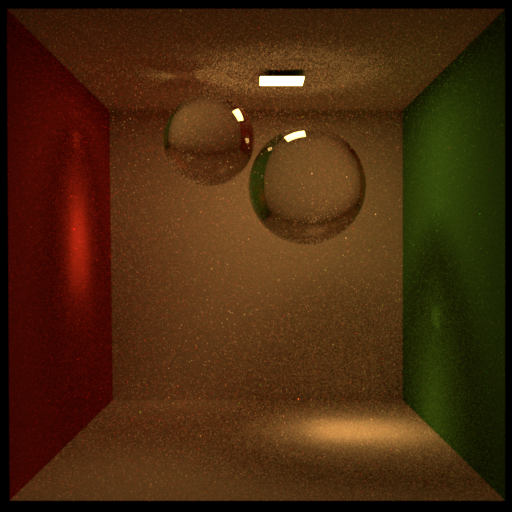
\includegraphics[width=0.5\textwidth]{bilder/kugelbox/nee&caches_200k20k2k_256spp.png}
\caption{NEE and IRC sampling: The IRCs handle the caustics, and NEE takes care of an overall smooth appearance.}
 \label{kugel_nee_caches}\end{figure}


 \begin{figure}[h!]
 \centering
 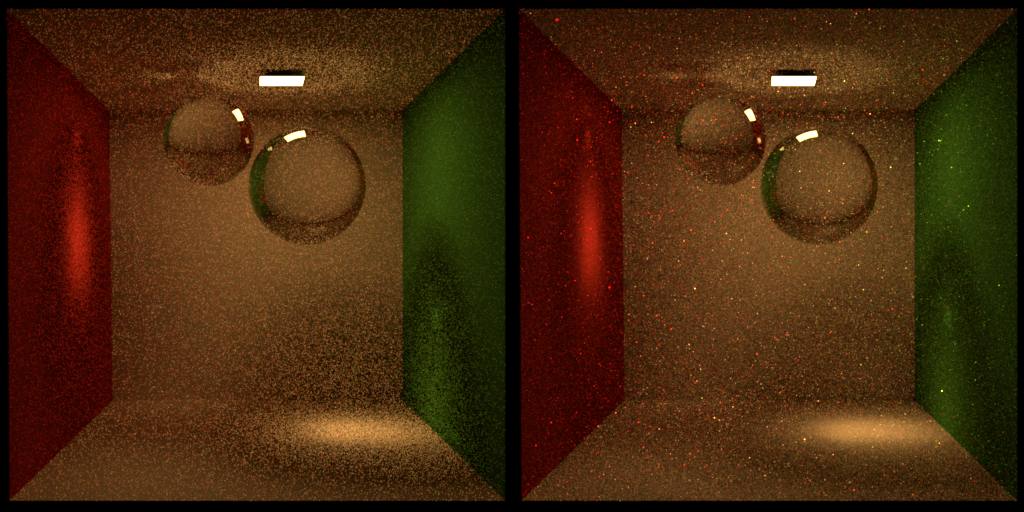
\includegraphics[width=1\textwidth]{bilder/kugelbox/bsdfcombos.png}
\caption{Left: NEE and BSDF sampling. In comparison to IRCs, BSDF sampling produces more noise in the caustics. The general noise produced by BSDF sampling consists of darker dots, while the noise of IRCs are colored sparks which can be cancelled out easier by NEE.\newline
Right: BSDF sampling and IRCs. The caustics look better than on the left, but the overall noise is worse.}
  \label{kugel_BSDF}\end{figure}

 \begin{figure}[h!]
 \centering
 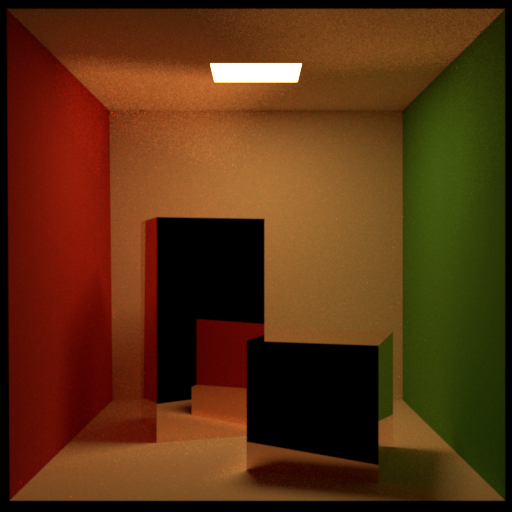
\includegraphics[width=0.5\textwidth]{bilder/spiegelbox/nee&caches_150k20k1k_128spp.png}
\caption{NEE and IRC sampling.}
  \label{spiegel_nee_caches}\end{figure}

 \begin{figure}[h!]
 \centering
 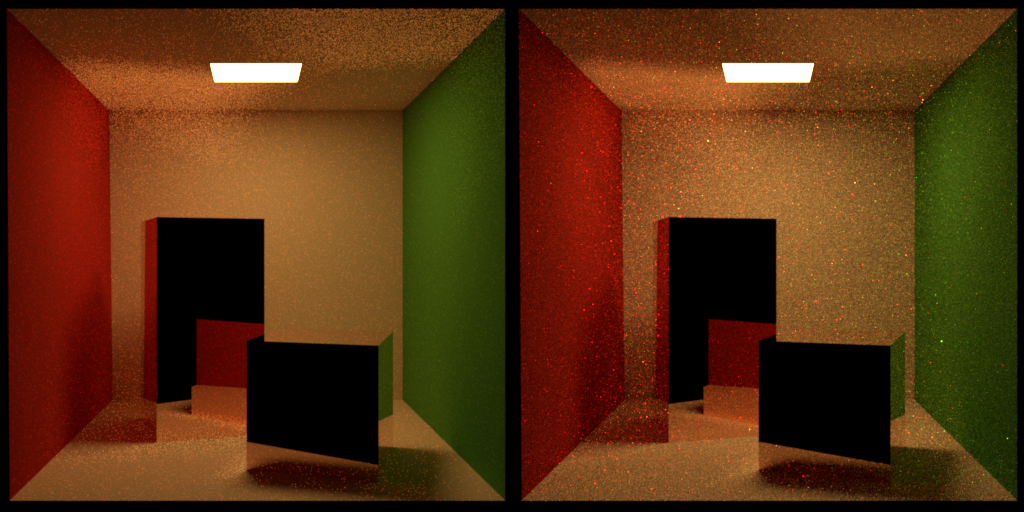
\includegraphics[width=1\textwidth]{bilder/spiegelbox/bsdfcombos_128spp.png}
\caption{Left: NEE and BSDF sampling. Just as with the glass spheres, the caustics show more noise than figure \ref{spiegel_nee_caches}. The noise on the walls is roughly the same, which might be the result of the brighter light source.\newline
Right: BSDF sampling and IRCs. While the caustics are smooth, there is notable noise from the IRCs.}
  \label{spiegel_BSDF}\end{figure}


 \begin{figure}[h!]
 \centering
 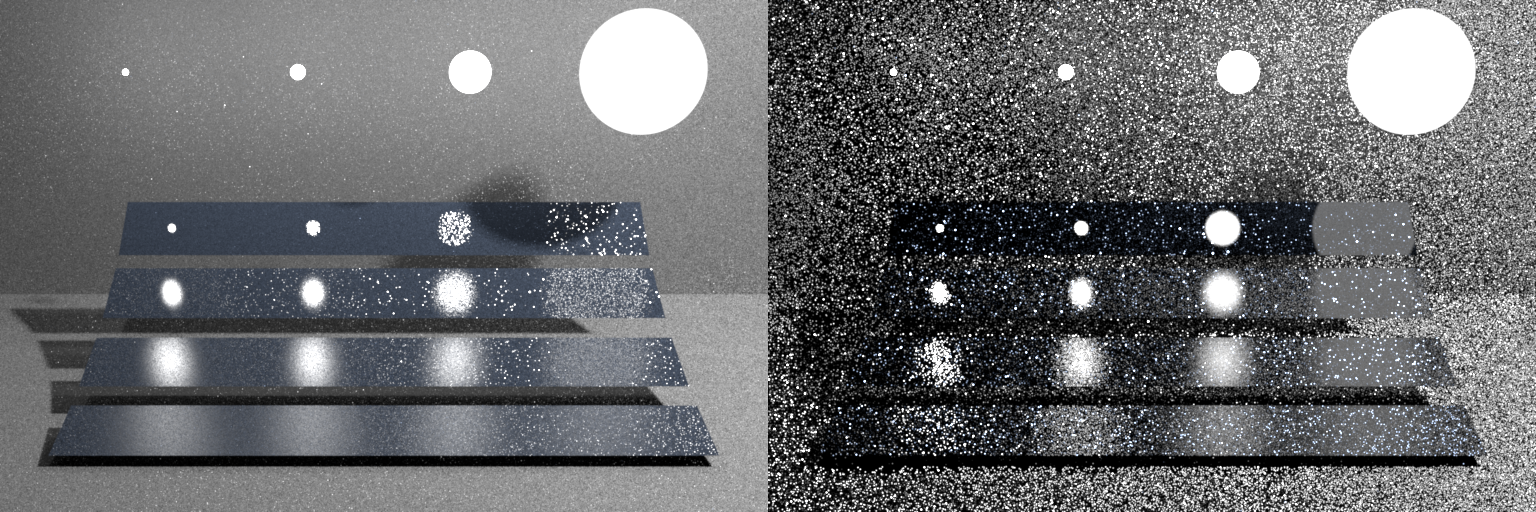
\includegraphics[width=1\textwidth]{bilder/veach/cachecombos_64spp.png}
\caption{Left: NEE and IRCs. Right: BSDF sampling and IRCs.}
  \label{veach_ircs}\end{figure}

 \begin{figure}[h!]
 \centering
 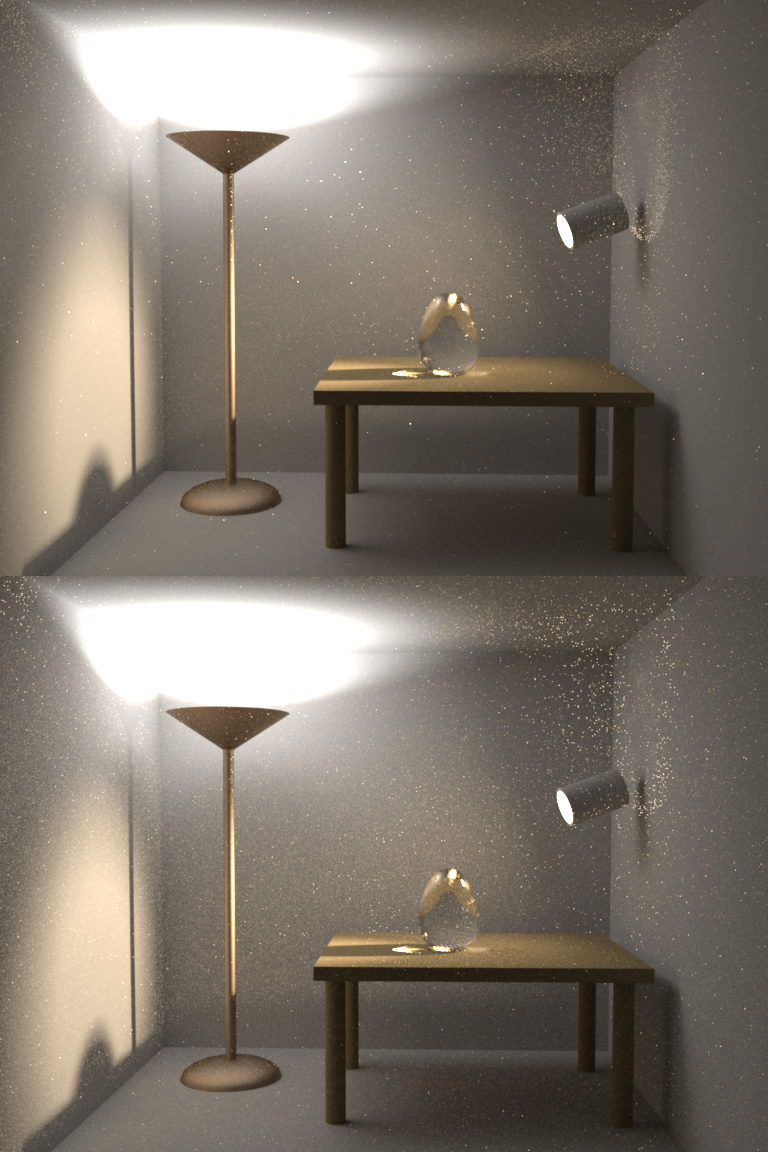
\includegraphics[width=0.7\textwidth]{bilder/bidir/vergleich.png}
\caption{Top: Rendered with NEE and IRCs, 250k photon paths ($\approx$ 1.500.000 photons), 30k caches, 2k photons per cache, 4096 samples per pixel.\newline
Bottom: Rendered with NEE and BSDF sampling, 4096 samples per pixel.}
  \label{bidir_ircs}\end{figure}



\clearpage



\subsection{Different Cache Configurations}\label{dcc}
In this section we investigate the impact of a different amount of photon paths, caches and photons per cache.\\
We found that environment map resolutions of $4\times 4$ and $8\times 8$ were too small, while a resolution $16\times 16$ produced decent results that $32\times 32$ was not able to improve.\\
As a limitation, we always created the same amount of camera caches (one for every $8\times 8$ pixel block). All additional caches were created from photons. The images below are rendered with NEE and IRC sampling, as this produced the best results.\\
The preprocessing time is proportional to the number of caches and number of photons per cache. The photon tracing pass itself is several orders of magnitude faster than filling the caches.


As it turns out, for simple scenes where most of the geometry is visible anyway the camera caches are mostly sufficient. However, there may appear artefacts along the edges. These can be removed by either picking one of the five closest caches with a better angle (see algorithm \ref{algopickcache}), or by adding more caches. For example, the glass sphere scene with camera caches only had 3768 caches and noticable artefacts along the edges within the caustic. These were gone when the same scene was rendered with 20k caches (figure \ref{artefacts}).



 \begin{figure}[h!]
 \centering
 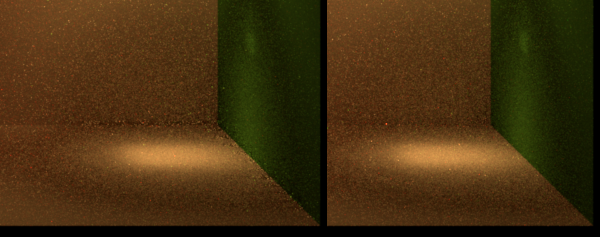
\includegraphics[width=0.8\textwidth]{bilder/kugelbox/caches/artefacts.png}
\caption{Left: camera caches only (3768).\newline
Right: 20k caches including camera caches.\newline
Note how the artefacts vanish on the left where the caustic ends.}
  \label{artefacts}\end{figure}

We also noticed that reducing the number of photon paths resulted in a general noise not unlike the noise from NEE $+$ BSDF sampling, while reducing the number of photons per cache generated a brighter, more colorful noise. Figure \ref{noises} illustrates two extremes that can be gradually improved by increasing the number of photon paths or photons per cache.


 \begin{figure}[h!]
 \centering
 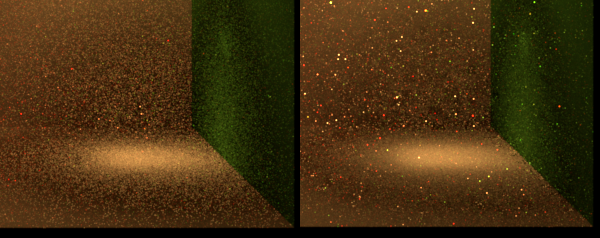
\includegraphics[width=0.8\textwidth]{bilder/kugelbox/caches/different_noises.png}
\caption{Left: 2k photon paths, 3768 caches, 2k photons per cache.\newline
Right: 200k photon paths, 3768 caches, 20 photons per cache.}
  \label{noises}\end{figure}

We settled on around 200k paths and 20k caches with 2k photons each for most of the images shown in section \ref{dcc}, as bigger numbers were not able to improve the images any further. Smaller numbers either produced noise (with less photon paths or photons per cache \ref{noises}) or caused artefacts along edges (too few caches \ref{artefacts}).\\
As a general rule, the number of photon paths should always be at least two orders of magnitude bigger than the number of photons per cache, if we want each cache to only use photons from its immediate surroundings. Our scenes contained an average of 4-8 photons per path. The more open the scene, the smaller this number gets. All our scenes were missing the wall towards the camera; within a completely closed scene there are most likely significantly more photons stored per path.




\subsection{Durations}
\label{durations}

We used an existing library to handle k-d trees and added a cdf to the caches so we could sample points faster using binary search, but apart from that we did not optimize our code in any way.\\
The images were rendered on an Intel i5-3570 CPU with 8GB RAM. The preprocessing of the caches runs in a single thread on one core. The path tracing is multithreaded over 4 cores. We believe the preprocessing step is well suited for parallelization as well, however the main part of the computation time is consumed by the path tracing step anyway.


We measured times for Mitsuba's default path tracer, our path tracer with NEE $+$ BSDF sampling (which does basically the same things as Mitsuba's version) and our path tracer with NEE $+$ IRC sampling. As BSDF $+$ IRC sampling produced the worst results for all of our test scenes, we don't have a detailed list of times for that approach, but it took roughly as long as NEE $+$ IRC sampling.\\
All times are given in minutes. We used 250k photon paths for 20k IRCs with 2500 photons each. The preprocessing time for the IRCs was 1 min and is included in the quoted times.

\begin{table}[h]
\begin{tabular}{|l|llll|}
\hline
                               & Samples per Pixel     & 256  & 512  & 4096  \\ \hline
\multirow{2}{*}{Glass Spheres} & NEE $+$ BSDF sampling & 1.4  & 2.8  & 22.6  \\
                               & NEE $+$ IRC sampling  & 10.9 & 20.7 & 152.1 \\ \hline
\multirow{3}{*}{Glass Egg}     & Mitsuba's path tracer & 3.5  & 7.4  & 58    \\
                               & NEE $+$ BSDF sampling & 4.4  & 8.5  & 71    \\
                               & NEE $+$ IRC sampling  & 19.0 & 37.0 & 281   \\ \hline
\end{tabular}
\end{table}

Observations:

\begin{itemize}
\item Our path tracer (with NEE and BSDF sampling) is not as optimized as Mitsuba's default version. So we believe there is still room for improving the render times.
\item The extra time for NEE $+$ IRC sampling is mainly the result of querying a k-d tree every time the ray intersects the scene. The smaller part is consumed by sampling a direction from the cache.
\item Picking one of the five closest caches resulted in approximately $50\%$ additional render time but no observable difference in the image. As a consequence we only used the closest cache for the listed measurements. All observed artefact problems can also be solved faster by using more caches.
\item For the Glass Spheres scene, NEE $+$ IRC sampling took about 10 times as long as NEE $+$ BSDF sampling, while it only took 4 times as long for the Glass Egg on Table. We assume that the relative overhead for NEE $+$ IRC sampling decreases further with increasing scene complexity, when more time is required to compute ray intersections with the scene.
\end{itemize}


\chapter{Related Work}
\label{chapter:relatedWork}

This chapter presents some alternative approaches to solve physically based light transport. We will start with Photon Mapping as a basis and introduce Final Gathering, Progressive Photon Mapping and Importance Driven Path Tracing as possible variations.\\
We also present Irradiance Caching, a technique that does not involve photon maps, but still is rather close to what we were trying to do.

\section{Photon Mapping}
\label{photon mapping}

Jensen and Christensen first introduced the idea to use photon maps in a bidirectional Monte Carlo ray tracing algorithm in 1994 (\cite{phomaps0}, \cite{phomaps1}). Over the years, many improvements and variations to the original approach were developed. Examples are Final Gathering \ref{final gathering}, Progressive Photon Mapping \ref{prophoma} and Importance Driven Path Tracing using the photon map \ref{idpt chapter}.

Most photon map - based algorithms consist of two passes: One pass to create the photon map, and one pass to render the image.\\
Chapter \ref{modified photon mapping} already explained how we created our photon map. The exact properties stored for each photon may vary, and sometimes several maps with different degrees of accuracy are built (e.g. \emph{caustic map} for photons that cause caustics, \emph{global photon map} for global illumination \cite[chapter 1.5]{phomaps2}), but the basic steps for creating a photon map are always the same.

Originally photon maps were used in a distributed ray tracing algorithm. The incident radiance is divided into separate parts, such as a direct illumination component ($L_e$), a component for caustics and a component for indirect illumination (\cite{phomaps2}). The caustics component and indirect illumination are evluated with a radiance estimate from the matching photon map.\\
Photon Mapping is biased but consistent - the average of many rendered images does not converge to the correct solution, while increasing the number of photons does.


\section{Final Gathering}
\label{final gathering}

Final Gathering is applied after the photon mapping pass and before (or while) the image is rendered. Direct illumination and caustics are handled as described before. To compute the indirect global illumination, we create a camera ray and take its first smooth intersection with the scene, called the \emph{final gather point}. Next, a number of \emph{final gather rays} is created over the upper hemisphere at the final gather point. At each first non-delta intersection of a final gather ray with the scene, the global photon map is evaluated to compute the indirect illumination along that ray. That way the total indirect illumination at the gather point can be estimated. The final gather rays are not traced any further.\\
Computing the indirect illumination for a gather point is relatively expensive, so depending on the scene it can be sufficient to create fewer final gather points and interpolate between them.\\
Many common render engines include final gathering to their photon-map based algorithms, since it is capable of efficiently producing accurate results for indirect illumination  (\cite{mentalray}, \cite{finalg}).

\section{Progressive Photon Mapping}
\label{prophoma}
The quality of conventional photon mapping is always limited by the memory space available for the photon map. The goal of progressive photon mapping is to use an arbitrarily high amount of photons without having to store all of them at the same time. \cite{ppm}\\
Progressive photon mapping begins with a ray tracing pass to identify and store all visible points (\emph{hit points}) in the scene. The hit points store their current radiance estimate, along with the number of photons and the radius used for that estimate. Thus the image can be rendered after any of the photon tracing passes.\\
The ray tracing pass is followed by an arbitrary number of photon tracing passes, where each pass increases the accuracy of the radiance estimate for the hit points. In the first photon tracing pass, a photon map is created and a radiance estimate is made for each hit point.  
Before each subsequent pass, the previous photon map can be deleted. The next pass creates a new photon map that is used to improve the previous radiance estimate. \cite{ppm} developed a procedure that increases the number of photons while simultaneously decreasing the radius used for the radiance estimate in each pass, in order to achieve a consistent (though still biased) algorithm.\\
Progressive photon mapping works especially well for scenes with SDS paths (light transport paths from specular to diffuse to specular surfaces).

\section{Irradiance Caching}
\label{irradiance caching}


Irradiance Caching was introduced 1988 by \cite{ward}. This approach is built upon the observation that indirect illumination changes smoothly on regular diffuse surfaces, while direct lighting may cause ``hard'' shadow boundaries. Irradiance Caching is designed for ray tracing algorithms where the rendering integral is divided into one part for direct lighting, one for specular reflection and refraction, and a third part for diffuse indirect lighting.\\
The first two can be approximated with a small number of rays, as they only depend on light from a small solid angle. However, integrating the indirect illumination is quite costly and can lead to an exponentially growing number of rays, since it has to consider light from all directions.

 Irradiance Caching aims to approximate and interpolate this diffuse indirect illumination through caches. The caches are created on the fly as necessary in order to avoid irrelevant computation of irradiance that is not needed for the image. They are rather sparsely distributed over the scene, such that regions with uniform irradiance have close to no caches, and regions with varying irradiance receive more.\\
 Each cache contains one value for the total irradiance around its position, and the irradiance values are interpolated from the surrounding caches for each ray intersection. The value directly contributes to the integral.\\
In contrast, our caches store multiple values for radiance from different directions and our algorithm uses theses values to extend a path.

Ward and Heckbert further suggested irradiance gradients \cite{ward2} to improve the interpolation between irradiance values. Another detailed overview on Irradiance Caching and derived methods is given in \cite[chapter 3]{irrc1}.

%http://www.rorydriscoll.com/2009/01/18/irradiance-caching-part-1/


\section{Importance Driven Path Tracing using the Photon Map}
\label{idpt chapter}
Of all previously explored techniques, Importance Driven Path Tracing is probably the closest thing to our IRCs. In this approach ``a rough estimate of the irradiance based on the photon map is combined with the local reflection model to construct more efficient probability density functions that can be used in an importance sampling scheme'' (\cite[abstract]{idpt}). The idea was introduced by Henrik Wann Jensen in 1995.

The first step here is photon mapping, where - as opposed to our approach - only photons that were reflected at least once are stored. Thus only indirect illumination is covered. In addition, a photon's flux is stored for different wavelengths.

\cite{idpt} skips the step of creating caches and starts rendering right after the photon map was created. Whenever they want to sample an outgoing camera path direction at some surface point $x$ with incoming direction $\omega_i$, they build a new pdf using the photon map:

\begin{itemize}
\item At first, the $N$ closest photons to $x$ are extracted from a k-d tree. 
\item Next, the contribution of each photon $p$ with flux $\Phi_p$ and incoming direction $\omega_p$ to the camera path arriving from $\omega_i$ at $x$ is computed as follows:
\begin{equation}
contribution = f_s(\omega_p,x,\omega_i) \cdot \Phi_p
\end{equation}
In contrast to our approach, this also includes the local BSDF to the pdf.
\item Then the direction $\omega_p$ of each photon $p$ is converted from a direction $\omega_p = (\theta_p,\phi_p)$ on the hemisphere to a point $(u,v)$ on the unit square.
\item The unit square is partitioned into $m\times n$ regions, and each photon's contribution is added to the corresponding part of the unit square.
\item The finalizing steps contain some scaling and eliminating all zeros in order to reach a valid pdf.
\item An outgoing direction for the path is then sampled from this local pdf.
\end{itemize}

Jensen was able to reduce the noise in an image through importance sampling with the photon map in comparison to no importance sampling at all.\\
However, the paper only used test scenes with mostly indirect illumination and - probably because it is relatively old - it did not contain images rendered with BSDF sampling and/or NEE.



\chapter{Conclusion and Future Work}
\label{chapter:Conclusion}

This thesis introduced caches for incident radiance as a possible sampling technique for Monte Carlo path tracing. A photon map was used to approximate incident radiance which was then stored in caches, so the photon map could be discarded before rendering. 

We showed that IRCs combined with NEE are a better choice for rendering caustics of all sorts in comparison to conventional path tracing with BSDF sampling and NEE. However, the advantages are restricted to caustics and ordinary diffuse surfaces; for direct lighting and more specular surfaces BSDF sampling and NEE produce better results.

Investigating the rendering times revealed that the preprocessing of the IRCs only consumes a small amount of the additional render time needed for NEE and IRC sampling. The rest of the time is distibuted about evenly between querying the k-d tree for the closest cache and sampling a texel and pdf value from it.\\
By decreasing the number of samples per pixel, we were able to generate images using NEE and IRC sampling that showed approximately the same quality and computation time as images rendered with NEE and BSDF sampling and a higher sample count. We also believe that the relative overhead for including IRCs decreases for a more complex geometry where more time is spent computing ray intersections.


%STIMMT NICHT MEHR For low sample counts per pixel, preprocessing the IRCs consumes a major part of the total rendering time. On the other hand, our test scenes showed that there soon comes a point where further increasing the number of photons (total or per cache) or caches does not further improve the quality. So as the number of samples per pixel increases, the share of computation time that goes towards preprocessing the caches decreases fast.\\

\null
We would like to make a few concluding suggestions for future improvement.

First of all, our implementation was rarely optimized. The preprocessing of the caches is highly suited for parallelization, we only neglected that because our test scenes were rather simple and therefore the benefit would have been minimal. Plus, the overall structure of our code was designed so that new features could be integrated and tested quickly, it was never optimized for a faster computation time.

Combining NEE, IRC sampling and BSDF sampling together could lead to a more robust algorithm that inherits the benefits from NEE and IRC sampling for caustics on smooth surfaces as well as the strengths of NEE and BSDF sampling for small light sources and more specular surfaces. The computation time should stay approximately the same as with NEE and IRC sampling, and the only modification necessary would be new MIS weights that are able to combine the one-sample model for BSDF and IRC sampling with the many-sample model for NEE and either BSDF or IRC sampling.

\newpage
Another option to improve the performance of NEE and IRC sampling on specular surfaces might be to include the BSDF when the cache's pdfs are created. A similar approach was already taken with Importance Driven Path Tracing \cite{idpt}, where each photon's energy was weighted with the BSDF for the outgoing direction and the incident direction of the current ray. This was possible because the pdfs were created as soon as a surface was hit, so information on the outgoing direction was available. Our caches are created before the image is rendered, so this method cannot be adopted as it stands.

%STIMMT, ist aber irrelevant: The relative amount of preprocessing time can be greatly reduced if more than one image of the same scene is rendered. As long as the geometry and lighting are static, all caches are valid for all new camera positions. Depending on the complexity of the scene, it might be wise to add some new camera caches for each new point of view, but we can skip the photon mapping step completely and reuse all of the old caches placed according to the photon distribution.

If necessary, the quality of the caches might be improved by filling them progressively with information that has to be computed anyway in order to render the image.\\
Progressive photon mapping \cite{ppm} already investigated how several photon tracing passes can iteratively increase the accuracy of an image rendered with photon mapping. Similarly, the pdf in the caches could be improved with information from multiple photon tracing passes.\\
It might even be possible to include the estimated incident radiance that is computed during path tracing. Thus the quality of the pdf in each texel could be increased progressively. However, the resolution of the environment maps used in the IRCs remains a limiting factor.

The concept of IRCs could also be used in a bidirectional path tracing algorithm. In addition to caching incident radiance, it should be possible to add analogous caches for importance from camera rays (instead of radiance from photon rays). Those caches could be employed to sample light paths, while the IRCs we introduced here could be used to sample camera paths.


%% ----------------
%% |   Appendix   |
%% ----------------
\cleardoublepage

%% --------------------
%% |   Bibliography   |
%% --------------------
\cleardoublepage
\phantomsection
\addcontentsline{toc}{chapter}{\bibname}

\iflanguage{english}
{\bibliographystyle{IEEEtranSA}}	% english style
{\bibliographystyle{babalpha-fl}}	% german style
												  
% Use IEEEtran for numeric references
\bibliographystyle{IEEEtranSA}

\bibliography{thesis}

\cleardoublepage
\vspace*{36\baselineskip}
\hbox to \textwidth{\hrulefill}
\par
\iflanguage{english}{I declare that I have developed and written the enclosed thesis completely by myself, and have not used sources or means without declaration in the text.}{Ich versichere wahrheitsgem\"a\ss, die Arbeit selbstst\"andig angefertigt, alle benutzten Hilfsmittel vollst\"andig und genau angegeben und alles kenntlich gemacht zu haben, was aus Arbeiten anderer unver\"andert oder mit Ab\"anderungen entnommen wurde.}

\textbf{Karlsruhe, 02.02.2015}
\vspace{1.5cm}

\dotfill\hspace*{8.0cm}\\
\hspace*{2cm}(\textbf{Alisa Jung}) %center name with hspace

\thispagestyle{empty}


\end{document}
